% =============================================================================
% 07-microprogrammed-control.tex — Week 7: Microprogrammed Control Unit Design
% (horizontal/vertical microinstructions; hardwired vs. microprogrammed)
%
% Course: Computer Organization and Architecture (PCC CS-401)
% Anchor reading: Mano Ch. 7 (control memory, microprogram counter, address
%                 sequencing, horizontal/vertical microinstruction formats);
%                 Stallings Ch. 16 (control unit design overview, microcode
%                 in practice)
%
% Compile with: /compile-latex CS401/07-microprogrammed-control
% =============================================================================

\documentclass[aspectratio=169]{beamer}
% =============================================================================
% Preambles/header.tex — shared LaTeX/Beamer preamble for this project
%
% Use from a Beamer lecture by prepending:
%     % =============================================================================
% Preambles/header.tex — shared LaTeX/Beamer preamble for this project
%
% Use from a Beamer lecture by prepending:
%     % =============================================================================
% Preambles/header.tex — shared LaTeX/Beamer preamble for this project
%
% Use from a Beamer lecture by prepending:
%     \input{header}
% and compiling with TEXINPUTS=../Preambles:$TEXINPUTS (the /compile-latex
% skill does this automatically).
%
% PALETTE CONTRACT. Color names defined here MUST match the names in
% Quarto/theme-template.scss so Beamer and Quarto renderings use the same
% palette. The scripts/check-palette-sync.sh script enforces this.
%
% To customize: edit the HEX values below AND the matching $variable in
% Quarto/theme-template.scss, then run scripts/check-palette-sync.sh.
%
% TITLE PAGE. A formal, serif (Libertine) title-page template is defined in
% the Beamer-only block below (\setbeamertemplate{title page}) -- title,
% subtitle, a thin gold rule, then \author/\institute/\date. Frametitle and
% body text remain on Beamer's sans-serif default. No SCSS counterpart is
% needed for this (font/layout only, no new colors).
% =============================================================================

% -----------------------------------------------------------------------------
% Engine detection + encoding
%
% Our /compile-latex skill uses XeLaTeX, where inputenc is unnecessary and
% can produce encoding warnings. Only load inputenc under pdfTeX.
% -----------------------------------------------------------------------------
\usepackage{iftex}
\ifPDFTeX
  \usepackage[utf8]{inputenc}
\fi

\usepackage{amsmath, amssymb, amsthm}
\usepackage{booktabs}
\usepackage{graphicx}

% -----------------------------------------------------------------------------
% Serif face for the title page (formal/academic look). Linux Libertine is
% XeLaTeX- and pdfTeX-safe and redefines \rmdefault, so \rmfamily picks it up
% everywhere \rmfamily is used explicitly. Body text and frametitles stay on
% Beamer's own sans-serif default (unaffected) -- only the title-page
% \setbeamerfont{...} overrides below opt in to \rmfamily.
% -----------------------------------------------------------------------------
\usepackage{libertine}

% -----------------------------------------------------------------------------
% PALETTE — mirrors Quarto/theme-template.scss variable names.
% Load xcolor and define colors BEFORE anything that references them
% (notably hyperref, hypersetup, and the Beamer color assignments).
% -----------------------------------------------------------------------------
\usepackage{xcolor}

\definecolor{primary-blue}{HTML}{012169}      % headings, accents
\definecolor{primary-gold}{HTML}{B9975B}      % emphasis, borders
\definecolor{highlight-yellow}{HTML}{F2A900}  % markers, alerts
\definecolor{light-bg}{HTML}{E8EDF5}          % title / section backgrounds
\definecolor{jet}{HTML}{1A1A1A}               % body text

% Semantic colors (used in diagrams and annotations)
\definecolor{positive}{HTML}{15803D}          % good / observed / identified
\definecolor{negative}{HTML}{B91C1C}          % bad / problematic / bias
\definecolor{neutral}{HTML}{525252}           % reference / context

% Highlight accents (match .hi-* classes in the SCSS)
\definecolor{hi-slate}{HTML}{314F4F}
\definecolor{hi-green}{HTML}{2E8B57}
\definecolor{hi-red}{HTML}{C41E3A}

% Semantic aliases so skill templates and snippets can write
% \textcolor{accent}{...} without hard-coding "primary-blue".
\colorlet{accent}{primary-blue}
\colorlet{accent2}{primary-gold}

% -----------------------------------------------------------------------------
% Hyperref — loaded AFTER xcolor + palette so link colors resolve.
% -----------------------------------------------------------------------------
\usepackage{hyperref}
\hypersetup{colorlinks=true, linkcolor=primary-blue, urlcolor=primary-blue,
            citecolor=primary-blue, pdfborder={0 0 0}}

% -----------------------------------------------------------------------------
% Course code — set once per deck (after \input{header}, before \begin{document})
% via \coursecode{CS401}. Shown in the footer on every slide so a deck's course
% is identifiable without opening the title page. Empty by default.
% -----------------------------------------------------------------------------
\makeatletter
\newcommand{\coursecode}[1]{\gdef\@coursecodetext{#1}}
\gdef\@coursecodetext{}
\makeatother

% -----------------------------------------------------------------------------
% Beamer theme assignments (only apply under Beamer).
%
% We detect Beamer via \@ifclassloaded{beamer}, which is the documented,
% non-internal way. This must be wrapped in \makeatletter/\makeatother
% because \@ifclassloaded contains an @-catcode character.
% -----------------------------------------------------------------------------
\makeatletter
\@ifclassloaded{beamer}{%
  \usefonttheme{professionalfonts}
  \setbeamercolor{structure}{fg=primary-blue}
  \setbeamercolor{frametitle}{fg=primary-blue}
  \setbeamercolor{title}{fg=primary-blue}
  \setbeamercolor{subtitle}{fg=primary-gold}
  \setbeamercolor{author}{fg=primary-blue}
  \setbeamercolor{institute}{fg=neutral}
  \setbeamercolor{date}{fg=primary-gold}
  \setbeamercolor{itemize item}{fg=primary-blue}
  \setbeamercolor{itemize subitem}{fg=primary-gold}
  \setbeamercolor{alerted text}{fg=primary-gold}
  \setbeamercolor{block title}{fg=white, bg=primary-blue}
  \setbeamercolor{block body}{bg=light-bg}
  % Semantic block variants: block=definition/concept (blue), exampleblock=
  % worked example (green/positive), alertblock=key takeaway or caution (gold).
  % Keep to <=2 colored boxes per slide across ALL three variants (INV-7).
  \setbeamercolor{block title example}{fg=white, bg=positive}
  \setbeamercolor{block body example}{bg=light-bg}
  \setbeamercolor{block title alerted}{fg=white, bg=primary-gold}
  \setbeamercolor{block body alerted}{bg=light-bg}

  % ---------------------------------------------------------------------------
  % Formal title page: serif (Libertine, via \rmfamily) for title-page
  % elements only. Body text, itemize, and frametitle are intentionally left
  % on Beamer's sans-serif default -- \usebeamerfont{title} is also what
  % \transitionslide (below) uses for its big centered text, so section
  % transitions pick up the same serif treatment for free.
  % ---------------------------------------------------------------------------
  \setbeamerfont{title}{family=\rmfamily, series=\bfseries, size=\Large}
  \setbeamerfont{subtitle}{family=\rmfamily, shape=\itshape, size=\normalsize}
  \setbeamerfont{author}{family=\rmfamily, size=\normalsize}
  \setbeamerfont{institute}{family=\rmfamily, size=\scriptsize}
  \setbeamerfont{date}{family=\rmfamily, size=\scriptsize}

  \setbeamertemplate{title page}{
    \vfill
    \begin{center}
      {\usebeamerfont{title}\usebeamercolor[fg]{title}\inserttitle\par}
      \vspace{0.15cm}
      {\usebeamerfont{subtitle}\usebeamercolor[fg]{subtitle}\insertsubtitle\par}
      \vspace{0.45cm}
      {\color{primary-gold}\rule{0.42\textwidth}{0.6pt}\par}
      \vspace{0.45cm}
      {\usebeamerfont{author}\usebeamercolor[fg]{author}\insertauthor\par}
      \vspace{0.35cm}
      {\usebeamerfont{institute}\usebeamercolor[fg]{institute}\insertinstitute\par}
      \vspace{0.35cm}
      {\usebeamerfont{date}\usebeamercolor[fg]{date}\insertdate\par}
    \end{center}
    \vfill
  }

  % Minimal footer: course code (left) + page X / N (right), no navigation clutter
  \setbeamertemplate{navigation symbols}{}
  \setbeamertemplate{footline}{%
    \color{neutral}\footnotesize\hspace{0.7em}\@coursecodetext\hfill
    \insertframenumber/\inserttotalframenumber\hspace{0.7em}\vspace{0.3em}}
}{}
\makeatother

% -----------------------------------------------------------------------------
% TikZ setup — libraries the snippet gallery uses
% -----------------------------------------------------------------------------
\usepackage{tikz}
\usetikzlibrary{arrows.meta, positioning, calc, decorations.pathreplacing,
                fit, shapes.geometric, backgrounds}

% Shared TikZ styles — snippets and hand-written diagrams can pick these up
% via `\begin{tikzpicture}[every node/.style={...}]` or by naming specific
% styles (e.g., `\node[dag-node] (X) at (0,0) {X};`).
\tikzset{
  % Node styles for causal DAGs and similar
  dag-node/.style = {
    draw=primary-blue, fill=light-bg, rounded corners=2pt,
    minimum width=1.2cm, minimum height=0.9cm, align=center, font=\small
  },
  decision-node/.style = {
    draw=primary-gold, fill=white, diamond, aspect=1.8,
    minimum width=1.8cm, minimum height=1.2cm, align=center, font=\small,
    inner sep=1pt
  },
  % Edge styles — observed vs counterfactual
  observed-edge/.style = {-{Latex[length=2.5mm]}, thick, draw=jet},
  counterfactual-edge/.style = {-{Latex[length=2.5mm]}, thick, draw=neutral, dashed},
  confound-edge/.style = {-{Latex[length=2.5mm]}, thick, draw=negative, dashed},
  % Data-point styles for plots
  observed-dot/.style = {fill=primary-blue, draw=primary-blue, circle, inner sep=1.2pt},
  counterfactual-dot/.style = {fill=white, draw=neutral, circle, inner sep=1.2pt}
}

% -----------------------------------------------------------------------------
% Convenience macros
% -----------------------------------------------------------------------------
\newcommand{\muted}[1]{\textcolor{neutral}{#1}}
\newcommand{\key}[1]{\textcolor{primary-gold}{\textbf{#1}}}
\newcommand{\good}[1]{\textcolor{positive}{#1}}
\newcommand{\bad}[1]{\textcolor{negative}{#1}}

% Standout frame macro: full-bleed dark background for section transitions.
% Beamer-only (uses \begin{frame}/\setbeamercolor/\usebeamerfont) -- do not
% call from an article-class file (e.g. Notes/<CODE>/*-notes.tex). \muted,
% \key, \good, \bad, and \coursecode above are plain xcolor/gdef and are
% safe to use from either class; verified when Notes/article-class support
% was added.
% Expand: \transitionslide{Your transition title}
\newcommand{\transitionslide}[1]{%
  \begingroup
  \setbeamercolor{background canvas}{bg=primary-blue}
  \begin{frame}[plain]
    \centering
    \vfill
    {\usebeamerfont{title}\color{white}\Large #1\par}
    \vfill
  \end{frame}
  \endgroup
}

% and compiling with TEXINPUTS=../Preambles:$TEXINPUTS (the /compile-latex
% skill does this automatically).
%
% PALETTE CONTRACT. Color names defined here MUST match the names in
% Quarto/theme-template.scss so Beamer and Quarto renderings use the same
% palette. The scripts/check-palette-sync.sh script enforces this.
%
% To customize: edit the HEX values below AND the matching $variable in
% Quarto/theme-template.scss, then run scripts/check-palette-sync.sh.
%
% TITLE PAGE. A formal, serif (Libertine) title-page template is defined in
% the Beamer-only block below (\setbeamertemplate{title page}) -- title,
% subtitle, a thin gold rule, then \author/\institute/\date. Frametitle and
% body text remain on Beamer's sans-serif default. No SCSS counterpart is
% needed for this (font/layout only, no new colors).
% =============================================================================

% -----------------------------------------------------------------------------
% Engine detection + encoding
%
% Our /compile-latex skill uses XeLaTeX, where inputenc is unnecessary and
% can produce encoding warnings. Only load inputenc under pdfTeX.
% -----------------------------------------------------------------------------
\usepackage{iftex}
\ifPDFTeX
  \usepackage[utf8]{inputenc}
\fi

\usepackage{amsmath, amssymb, amsthm}
\usepackage{booktabs}
\usepackage{graphicx}

% -----------------------------------------------------------------------------
% Serif face for the title page (formal/academic look). Linux Libertine is
% XeLaTeX- and pdfTeX-safe and redefines \rmdefault, so \rmfamily picks it up
% everywhere \rmfamily is used explicitly. Body text and frametitles stay on
% Beamer's own sans-serif default (unaffected) -- only the title-page
% \setbeamerfont{...} overrides below opt in to \rmfamily.
% -----------------------------------------------------------------------------
\usepackage{libertine}

% -----------------------------------------------------------------------------
% PALETTE — mirrors Quarto/theme-template.scss variable names.
% Load xcolor and define colors BEFORE anything that references them
% (notably hyperref, hypersetup, and the Beamer color assignments).
% -----------------------------------------------------------------------------
\usepackage{xcolor}

\definecolor{primary-blue}{HTML}{012169}      % headings, accents
\definecolor{primary-gold}{HTML}{B9975B}      % emphasis, borders
\definecolor{highlight-yellow}{HTML}{F2A900}  % markers, alerts
\definecolor{light-bg}{HTML}{E8EDF5}          % title / section backgrounds
\definecolor{jet}{HTML}{1A1A1A}               % body text

% Semantic colors (used in diagrams and annotations)
\definecolor{positive}{HTML}{15803D}          % good / observed / identified
\definecolor{negative}{HTML}{B91C1C}          % bad / problematic / bias
\definecolor{neutral}{HTML}{525252}           % reference / context

% Highlight accents (match .hi-* classes in the SCSS)
\definecolor{hi-slate}{HTML}{314F4F}
\definecolor{hi-green}{HTML}{2E8B57}
\definecolor{hi-red}{HTML}{C41E3A}

% Semantic aliases so skill templates and snippets can write
% \textcolor{accent}{...} without hard-coding "primary-blue".
\colorlet{accent}{primary-blue}
\colorlet{accent2}{primary-gold}

% -----------------------------------------------------------------------------
% Hyperref — loaded AFTER xcolor + palette so link colors resolve.
% -----------------------------------------------------------------------------
\usepackage{hyperref}
\hypersetup{colorlinks=true, linkcolor=primary-blue, urlcolor=primary-blue,
            citecolor=primary-blue, pdfborder={0 0 0}}

% -----------------------------------------------------------------------------
% Course code — set once per deck (after % =============================================================================
% Preambles/header.tex — shared LaTeX/Beamer preamble for this project
%
% Use from a Beamer lecture by prepending:
%     \input{header}
% and compiling with TEXINPUTS=../Preambles:$TEXINPUTS (the /compile-latex
% skill does this automatically).
%
% PALETTE CONTRACT. Color names defined here MUST match the names in
% Quarto/theme-template.scss so Beamer and Quarto renderings use the same
% palette. The scripts/check-palette-sync.sh script enforces this.
%
% To customize: edit the HEX values below AND the matching $variable in
% Quarto/theme-template.scss, then run scripts/check-palette-sync.sh.
%
% TITLE PAGE. A formal, serif (Libertine) title-page template is defined in
% the Beamer-only block below (\setbeamertemplate{title page}) -- title,
% subtitle, a thin gold rule, then \author/\institute/\date. Frametitle and
% body text remain on Beamer's sans-serif default. No SCSS counterpart is
% needed for this (font/layout only, no new colors).
% =============================================================================

% -----------------------------------------------------------------------------
% Engine detection + encoding
%
% Our /compile-latex skill uses XeLaTeX, where inputenc is unnecessary and
% can produce encoding warnings. Only load inputenc under pdfTeX.
% -----------------------------------------------------------------------------
\usepackage{iftex}
\ifPDFTeX
  \usepackage[utf8]{inputenc}
\fi

\usepackage{amsmath, amssymb, amsthm}
\usepackage{booktabs}
\usepackage{graphicx}

% -----------------------------------------------------------------------------
% Serif face for the title page (formal/academic look). Linux Libertine is
% XeLaTeX- and pdfTeX-safe and redefines \rmdefault, so \rmfamily picks it up
% everywhere \rmfamily is used explicitly. Body text and frametitles stay on
% Beamer's own sans-serif default (unaffected) -- only the title-page
% \setbeamerfont{...} overrides below opt in to \rmfamily.
% -----------------------------------------------------------------------------
\usepackage{libertine}

% -----------------------------------------------------------------------------
% PALETTE — mirrors Quarto/theme-template.scss variable names.
% Load xcolor and define colors BEFORE anything that references them
% (notably hyperref, hypersetup, and the Beamer color assignments).
% -----------------------------------------------------------------------------
\usepackage{xcolor}

\definecolor{primary-blue}{HTML}{012169}      % headings, accents
\definecolor{primary-gold}{HTML}{B9975B}      % emphasis, borders
\definecolor{highlight-yellow}{HTML}{F2A900}  % markers, alerts
\definecolor{light-bg}{HTML}{E8EDF5}          % title / section backgrounds
\definecolor{jet}{HTML}{1A1A1A}               % body text

% Semantic colors (used in diagrams and annotations)
\definecolor{positive}{HTML}{15803D}          % good / observed / identified
\definecolor{negative}{HTML}{B91C1C}          % bad / problematic / bias
\definecolor{neutral}{HTML}{525252}           % reference / context

% Highlight accents (match .hi-* classes in the SCSS)
\definecolor{hi-slate}{HTML}{314F4F}
\definecolor{hi-green}{HTML}{2E8B57}
\definecolor{hi-red}{HTML}{C41E3A}

% Semantic aliases so skill templates and snippets can write
% \textcolor{accent}{...} without hard-coding "primary-blue".
\colorlet{accent}{primary-blue}
\colorlet{accent2}{primary-gold}

% -----------------------------------------------------------------------------
% Hyperref — loaded AFTER xcolor + palette so link colors resolve.
% -----------------------------------------------------------------------------
\usepackage{hyperref}
\hypersetup{colorlinks=true, linkcolor=primary-blue, urlcolor=primary-blue,
            citecolor=primary-blue, pdfborder={0 0 0}}

% -----------------------------------------------------------------------------
% Course code — set once per deck (after \input{header}, before \begin{document})
% via \coursecode{CS401}. Shown in the footer on every slide so a deck's course
% is identifiable without opening the title page. Empty by default.
% -----------------------------------------------------------------------------
\makeatletter
\newcommand{\coursecode}[1]{\gdef\@coursecodetext{#1}}
\gdef\@coursecodetext{}
\makeatother

% -----------------------------------------------------------------------------
% Beamer theme assignments (only apply under Beamer).
%
% We detect Beamer via \@ifclassloaded{beamer}, which is the documented,
% non-internal way. This must be wrapped in \makeatletter/\makeatother
% because \@ifclassloaded contains an @-catcode character.
% -----------------------------------------------------------------------------
\makeatletter
\@ifclassloaded{beamer}{%
  \usefonttheme{professionalfonts}
  \setbeamercolor{structure}{fg=primary-blue}
  \setbeamercolor{frametitle}{fg=primary-blue}
  \setbeamercolor{title}{fg=primary-blue}
  \setbeamercolor{subtitle}{fg=primary-gold}
  \setbeamercolor{author}{fg=primary-blue}
  \setbeamercolor{institute}{fg=neutral}
  \setbeamercolor{date}{fg=primary-gold}
  \setbeamercolor{itemize item}{fg=primary-blue}
  \setbeamercolor{itemize subitem}{fg=primary-gold}
  \setbeamercolor{alerted text}{fg=primary-gold}
  \setbeamercolor{block title}{fg=white, bg=primary-blue}
  \setbeamercolor{block body}{bg=light-bg}
  % Semantic block variants: block=definition/concept (blue), exampleblock=
  % worked example (green/positive), alertblock=key takeaway or caution (gold).
  % Keep to <=2 colored boxes per slide across ALL three variants (INV-7).
  \setbeamercolor{block title example}{fg=white, bg=positive}
  \setbeamercolor{block body example}{bg=light-bg}
  \setbeamercolor{block title alerted}{fg=white, bg=primary-gold}
  \setbeamercolor{block body alerted}{bg=light-bg}

  % ---------------------------------------------------------------------------
  % Formal title page: serif (Libertine, via \rmfamily) for title-page
  % elements only. Body text, itemize, and frametitle are intentionally left
  % on Beamer's sans-serif default -- \usebeamerfont{title} is also what
  % \transitionslide (below) uses for its big centered text, so section
  % transitions pick up the same serif treatment for free.
  % ---------------------------------------------------------------------------
  \setbeamerfont{title}{family=\rmfamily, series=\bfseries, size=\Large}
  \setbeamerfont{subtitle}{family=\rmfamily, shape=\itshape, size=\normalsize}
  \setbeamerfont{author}{family=\rmfamily, size=\normalsize}
  \setbeamerfont{institute}{family=\rmfamily, size=\scriptsize}
  \setbeamerfont{date}{family=\rmfamily, size=\scriptsize}

  \setbeamertemplate{title page}{
    \vfill
    \begin{center}
      {\usebeamerfont{title}\usebeamercolor[fg]{title}\inserttitle\par}
      \vspace{0.15cm}
      {\usebeamerfont{subtitle}\usebeamercolor[fg]{subtitle}\insertsubtitle\par}
      \vspace{0.45cm}
      {\color{primary-gold}\rule{0.42\textwidth}{0.6pt}\par}
      \vspace{0.45cm}
      {\usebeamerfont{author}\usebeamercolor[fg]{author}\insertauthor\par}
      \vspace{0.35cm}
      {\usebeamerfont{institute}\usebeamercolor[fg]{institute}\insertinstitute\par}
      \vspace{0.35cm}
      {\usebeamerfont{date}\usebeamercolor[fg]{date}\insertdate\par}
    \end{center}
    \vfill
  }

  % Minimal footer: course code (left) + page X / N (right), no navigation clutter
  \setbeamertemplate{navigation symbols}{}
  \setbeamertemplate{footline}{%
    \color{neutral}\footnotesize\hspace{0.7em}\@coursecodetext\hfill
    \insertframenumber/\inserttotalframenumber\hspace{0.7em}\vspace{0.3em}}
}{}
\makeatother

% -----------------------------------------------------------------------------
% TikZ setup — libraries the snippet gallery uses
% -----------------------------------------------------------------------------
\usepackage{tikz}
\usetikzlibrary{arrows.meta, positioning, calc, decorations.pathreplacing,
                fit, shapes.geometric, backgrounds}

% Shared TikZ styles — snippets and hand-written diagrams can pick these up
% via `\begin{tikzpicture}[every node/.style={...}]` or by naming specific
% styles (e.g., `\node[dag-node] (X) at (0,0) {X};`).
\tikzset{
  % Node styles for causal DAGs and similar
  dag-node/.style = {
    draw=primary-blue, fill=light-bg, rounded corners=2pt,
    minimum width=1.2cm, minimum height=0.9cm, align=center, font=\small
  },
  decision-node/.style = {
    draw=primary-gold, fill=white, diamond, aspect=1.8,
    minimum width=1.8cm, minimum height=1.2cm, align=center, font=\small,
    inner sep=1pt
  },
  % Edge styles — observed vs counterfactual
  observed-edge/.style = {-{Latex[length=2.5mm]}, thick, draw=jet},
  counterfactual-edge/.style = {-{Latex[length=2.5mm]}, thick, draw=neutral, dashed},
  confound-edge/.style = {-{Latex[length=2.5mm]}, thick, draw=negative, dashed},
  % Data-point styles for plots
  observed-dot/.style = {fill=primary-blue, draw=primary-blue, circle, inner sep=1.2pt},
  counterfactual-dot/.style = {fill=white, draw=neutral, circle, inner sep=1.2pt}
}

% -----------------------------------------------------------------------------
% Convenience macros
% -----------------------------------------------------------------------------
\newcommand{\muted}[1]{\textcolor{neutral}{#1}}
\newcommand{\key}[1]{\textcolor{primary-gold}{\textbf{#1}}}
\newcommand{\good}[1]{\textcolor{positive}{#1}}
\newcommand{\bad}[1]{\textcolor{negative}{#1}}

% Standout frame macro: full-bleed dark background for section transitions.
% Beamer-only (uses \begin{frame}/\setbeamercolor/\usebeamerfont) -- do not
% call from an article-class file (e.g. Notes/<CODE>/*-notes.tex). \muted,
% \key, \good, \bad, and \coursecode above are plain xcolor/gdef and are
% safe to use from either class; verified when Notes/article-class support
% was added.
% Expand: \transitionslide{Your transition title}
\newcommand{\transitionslide}[1]{%
  \begingroup
  \setbeamercolor{background canvas}{bg=primary-blue}
  \begin{frame}[plain]
    \centering
    \vfill
    {\usebeamerfont{title}\color{white}\Large #1\par}
    \vfill
  \end{frame}
  \endgroup
}
, before \begin{document})
% via \coursecode{CS401}. Shown in the footer on every slide so a deck's course
% is identifiable without opening the title page. Empty by default.
% -----------------------------------------------------------------------------
\makeatletter
\newcommand{\coursecode}[1]{\gdef\@coursecodetext{#1}}
\gdef\@coursecodetext{}
\makeatother

% -----------------------------------------------------------------------------
% Beamer theme assignments (only apply under Beamer).
%
% We detect Beamer via \@ifclassloaded{beamer}, which is the documented,
% non-internal way. This must be wrapped in \makeatletter/\makeatother
% because \@ifclassloaded contains an @-catcode character.
% -----------------------------------------------------------------------------
\makeatletter
\@ifclassloaded{beamer}{%
  \usefonttheme{professionalfonts}
  \setbeamercolor{structure}{fg=primary-blue}
  \setbeamercolor{frametitle}{fg=primary-blue}
  \setbeamercolor{title}{fg=primary-blue}
  \setbeamercolor{subtitle}{fg=primary-gold}
  \setbeamercolor{author}{fg=primary-blue}
  \setbeamercolor{institute}{fg=neutral}
  \setbeamercolor{date}{fg=primary-gold}
  \setbeamercolor{itemize item}{fg=primary-blue}
  \setbeamercolor{itemize subitem}{fg=primary-gold}
  \setbeamercolor{alerted text}{fg=primary-gold}
  \setbeamercolor{block title}{fg=white, bg=primary-blue}
  \setbeamercolor{block body}{bg=light-bg}
  % Semantic block variants: block=definition/concept (blue), exampleblock=
  % worked example (green/positive), alertblock=key takeaway or caution (gold).
  % Keep to <=2 colored boxes per slide across ALL three variants (INV-7).
  \setbeamercolor{block title example}{fg=white, bg=positive}
  \setbeamercolor{block body example}{bg=light-bg}
  \setbeamercolor{block title alerted}{fg=white, bg=primary-gold}
  \setbeamercolor{block body alerted}{bg=light-bg}

  % ---------------------------------------------------------------------------
  % Formal title page: serif (Libertine, via \rmfamily) for title-page
  % elements only. Body text, itemize, and frametitle are intentionally left
  % on Beamer's sans-serif default -- \usebeamerfont{title} is also what
  % \transitionslide (below) uses for its big centered text, so section
  % transitions pick up the same serif treatment for free.
  % ---------------------------------------------------------------------------
  \setbeamerfont{title}{family=\rmfamily, series=\bfseries, size=\Large}
  \setbeamerfont{subtitle}{family=\rmfamily, shape=\itshape, size=\normalsize}
  \setbeamerfont{author}{family=\rmfamily, size=\normalsize}
  \setbeamerfont{institute}{family=\rmfamily, size=\scriptsize}
  \setbeamerfont{date}{family=\rmfamily, size=\scriptsize}

  \setbeamertemplate{title page}{
    \vfill
    \begin{center}
      {\usebeamerfont{title}\usebeamercolor[fg]{title}\inserttitle\par}
      \vspace{0.15cm}
      {\usebeamerfont{subtitle}\usebeamercolor[fg]{subtitle}\insertsubtitle\par}
      \vspace{0.45cm}
      {\color{primary-gold}\rule{0.42\textwidth}{0.6pt}\par}
      \vspace{0.45cm}
      {\usebeamerfont{author}\usebeamercolor[fg]{author}\insertauthor\par}
      \vspace{0.35cm}
      {\usebeamerfont{institute}\usebeamercolor[fg]{institute}\insertinstitute\par}
      \vspace{0.35cm}
      {\usebeamerfont{date}\usebeamercolor[fg]{date}\insertdate\par}
    \end{center}
    \vfill
  }

  % Minimal footer: course code (left) + page X / N (right), no navigation clutter
  \setbeamertemplate{navigation symbols}{}
  \setbeamertemplate{footline}{%
    \color{neutral}\footnotesize\hspace{0.7em}\@coursecodetext\hfill
    \insertframenumber/\inserttotalframenumber\hspace{0.7em}\vspace{0.3em}}
}{}
\makeatother

% -----------------------------------------------------------------------------
% TikZ setup — libraries the snippet gallery uses
% -----------------------------------------------------------------------------
\usepackage{tikz}
\usetikzlibrary{arrows.meta, positioning, calc, decorations.pathreplacing,
                fit, shapes.geometric, backgrounds}

% Shared TikZ styles — snippets and hand-written diagrams can pick these up
% via `\begin{tikzpicture}[every node/.style={...}]` or by naming specific
% styles (e.g., `\node[dag-node] (X) at (0,0) {X};`).
\tikzset{
  % Node styles for causal DAGs and similar
  dag-node/.style = {
    draw=primary-blue, fill=light-bg, rounded corners=2pt,
    minimum width=1.2cm, minimum height=0.9cm, align=center, font=\small
  },
  decision-node/.style = {
    draw=primary-gold, fill=white, diamond, aspect=1.8,
    minimum width=1.8cm, minimum height=1.2cm, align=center, font=\small,
    inner sep=1pt
  },
  % Edge styles — observed vs counterfactual
  observed-edge/.style = {-{Latex[length=2.5mm]}, thick, draw=jet},
  counterfactual-edge/.style = {-{Latex[length=2.5mm]}, thick, draw=neutral, dashed},
  confound-edge/.style = {-{Latex[length=2.5mm]}, thick, draw=negative, dashed},
  % Data-point styles for plots
  observed-dot/.style = {fill=primary-blue, draw=primary-blue, circle, inner sep=1.2pt},
  counterfactual-dot/.style = {fill=white, draw=neutral, circle, inner sep=1.2pt}
}

% -----------------------------------------------------------------------------
% Convenience macros
% -----------------------------------------------------------------------------
\newcommand{\muted}[1]{\textcolor{neutral}{#1}}
\newcommand{\key}[1]{\textcolor{primary-gold}{\textbf{#1}}}
\newcommand{\good}[1]{\textcolor{positive}{#1}}
\newcommand{\bad}[1]{\textcolor{negative}{#1}}

% Standout frame macro: full-bleed dark background for section transitions.
% Beamer-only (uses \begin{frame}/\setbeamercolor/\usebeamerfont) -- do not
% call from an article-class file (e.g. Notes/<CODE>/*-notes.tex). \muted,
% \key, \good, \bad, and \coursecode above are plain xcolor/gdef and are
% safe to use from either class; verified when Notes/article-class support
% was added.
% Expand: \transitionslide{Your transition title}
\newcommand{\transitionslide}[1]{%
  \begingroup
  \setbeamercolor{background canvas}{bg=primary-blue}
  \begin{frame}[plain]
    \centering
    \vfill
    {\usebeamerfont{title}\color{white}\Large #1\par}
    \vfill
  \end{frame}
  \endgroup
}

% and compiling with TEXINPUTS=../Preambles:$TEXINPUTS (the /compile-latex
% skill does this automatically).
%
% PALETTE CONTRACT. Color names defined here MUST match the names in
% Quarto/theme-template.scss so Beamer and Quarto renderings use the same
% palette. The scripts/check-palette-sync.sh script enforces this.
%
% To customize: edit the HEX values below AND the matching $variable in
% Quarto/theme-template.scss, then run scripts/check-palette-sync.sh.
%
% TITLE PAGE. A formal, serif (Libertine) title-page template is defined in
% the Beamer-only block below (\setbeamertemplate{title page}) -- title,
% subtitle, a thin gold rule, then \author/\institute/\date. Frametitle and
% body text remain on Beamer's sans-serif default. No SCSS counterpart is
% needed for this (font/layout only, no new colors).
% =============================================================================

% -----------------------------------------------------------------------------
% Engine detection + encoding
%
% Our /compile-latex skill uses XeLaTeX, where inputenc is unnecessary and
% can produce encoding warnings. Only load inputenc under pdfTeX.
% -----------------------------------------------------------------------------
\usepackage{iftex}
\ifPDFTeX
  \usepackage[utf8]{inputenc}
\fi

\usepackage{amsmath, amssymb, amsthm}
\usepackage{booktabs}
\usepackage{graphicx}

% -----------------------------------------------------------------------------
% Serif face for the title page (formal/academic look). Linux Libertine is
% XeLaTeX- and pdfTeX-safe and redefines \rmdefault, so \rmfamily picks it up
% everywhere \rmfamily is used explicitly. Body text and frametitles stay on
% Beamer's own sans-serif default (unaffected) -- only the title-page
% \setbeamerfont{...} overrides below opt in to \rmfamily.
% -----------------------------------------------------------------------------
\usepackage{libertine}

% -----------------------------------------------------------------------------
% PALETTE — mirrors Quarto/theme-template.scss variable names.
% Load xcolor and define colors BEFORE anything that references them
% (notably hyperref, hypersetup, and the Beamer color assignments).
% -----------------------------------------------------------------------------
\usepackage{xcolor}

\definecolor{primary-blue}{HTML}{012169}      % headings, accents
\definecolor{primary-gold}{HTML}{B9975B}      % emphasis, borders
\definecolor{highlight-yellow}{HTML}{F2A900}  % markers, alerts
\definecolor{light-bg}{HTML}{E8EDF5}          % title / section backgrounds
\definecolor{jet}{HTML}{1A1A1A}               % body text

% Semantic colors (used in diagrams and annotations)
\definecolor{positive}{HTML}{15803D}          % good / observed / identified
\definecolor{negative}{HTML}{B91C1C}          % bad / problematic / bias
\definecolor{neutral}{HTML}{525252}           % reference / context

% Highlight accents (match .hi-* classes in the SCSS)
\definecolor{hi-slate}{HTML}{314F4F}
\definecolor{hi-green}{HTML}{2E8B57}
\definecolor{hi-red}{HTML}{C41E3A}

% Semantic aliases so skill templates and snippets can write
% \textcolor{accent}{...} without hard-coding "primary-blue".
\colorlet{accent}{primary-blue}
\colorlet{accent2}{primary-gold}

% -----------------------------------------------------------------------------
% Hyperref — loaded AFTER xcolor + palette so link colors resolve.
% -----------------------------------------------------------------------------
\usepackage{hyperref}
\hypersetup{colorlinks=true, linkcolor=primary-blue, urlcolor=primary-blue,
            citecolor=primary-blue, pdfborder={0 0 0}}

% -----------------------------------------------------------------------------
% Course code — set once per deck (after % =============================================================================
% Preambles/header.tex — shared LaTeX/Beamer preamble for this project
%
% Use from a Beamer lecture by prepending:
%     % =============================================================================
% Preambles/header.tex — shared LaTeX/Beamer preamble for this project
%
% Use from a Beamer lecture by prepending:
%     \input{header}
% and compiling with TEXINPUTS=../Preambles:$TEXINPUTS (the /compile-latex
% skill does this automatically).
%
% PALETTE CONTRACT. Color names defined here MUST match the names in
% Quarto/theme-template.scss so Beamer and Quarto renderings use the same
% palette. The scripts/check-palette-sync.sh script enforces this.
%
% To customize: edit the HEX values below AND the matching $variable in
% Quarto/theme-template.scss, then run scripts/check-palette-sync.sh.
%
% TITLE PAGE. A formal, serif (Libertine) title-page template is defined in
% the Beamer-only block below (\setbeamertemplate{title page}) -- title,
% subtitle, a thin gold rule, then \author/\institute/\date. Frametitle and
% body text remain on Beamer's sans-serif default. No SCSS counterpart is
% needed for this (font/layout only, no new colors).
% =============================================================================

% -----------------------------------------------------------------------------
% Engine detection + encoding
%
% Our /compile-latex skill uses XeLaTeX, where inputenc is unnecessary and
% can produce encoding warnings. Only load inputenc under pdfTeX.
% -----------------------------------------------------------------------------
\usepackage{iftex}
\ifPDFTeX
  \usepackage[utf8]{inputenc}
\fi

\usepackage{amsmath, amssymb, amsthm}
\usepackage{booktabs}
\usepackage{graphicx}

% -----------------------------------------------------------------------------
% Serif face for the title page (formal/academic look). Linux Libertine is
% XeLaTeX- and pdfTeX-safe and redefines \rmdefault, so \rmfamily picks it up
% everywhere \rmfamily is used explicitly. Body text and frametitles stay on
% Beamer's own sans-serif default (unaffected) -- only the title-page
% \setbeamerfont{...} overrides below opt in to \rmfamily.
% -----------------------------------------------------------------------------
\usepackage{libertine}

% -----------------------------------------------------------------------------
% PALETTE — mirrors Quarto/theme-template.scss variable names.
% Load xcolor and define colors BEFORE anything that references them
% (notably hyperref, hypersetup, and the Beamer color assignments).
% -----------------------------------------------------------------------------
\usepackage{xcolor}

\definecolor{primary-blue}{HTML}{012169}      % headings, accents
\definecolor{primary-gold}{HTML}{B9975B}      % emphasis, borders
\definecolor{highlight-yellow}{HTML}{F2A900}  % markers, alerts
\definecolor{light-bg}{HTML}{E8EDF5}          % title / section backgrounds
\definecolor{jet}{HTML}{1A1A1A}               % body text

% Semantic colors (used in diagrams and annotations)
\definecolor{positive}{HTML}{15803D}          % good / observed / identified
\definecolor{negative}{HTML}{B91C1C}          % bad / problematic / bias
\definecolor{neutral}{HTML}{525252}           % reference / context

% Highlight accents (match .hi-* classes in the SCSS)
\definecolor{hi-slate}{HTML}{314F4F}
\definecolor{hi-green}{HTML}{2E8B57}
\definecolor{hi-red}{HTML}{C41E3A}

% Semantic aliases so skill templates and snippets can write
% \textcolor{accent}{...} without hard-coding "primary-blue".
\colorlet{accent}{primary-blue}
\colorlet{accent2}{primary-gold}

% -----------------------------------------------------------------------------
% Hyperref — loaded AFTER xcolor + palette so link colors resolve.
% -----------------------------------------------------------------------------
\usepackage{hyperref}
\hypersetup{colorlinks=true, linkcolor=primary-blue, urlcolor=primary-blue,
            citecolor=primary-blue, pdfborder={0 0 0}}

% -----------------------------------------------------------------------------
% Course code — set once per deck (after \input{header}, before \begin{document})
% via \coursecode{CS401}. Shown in the footer on every slide so a deck's course
% is identifiable without opening the title page. Empty by default.
% -----------------------------------------------------------------------------
\makeatletter
\newcommand{\coursecode}[1]{\gdef\@coursecodetext{#1}}
\gdef\@coursecodetext{}
\makeatother

% -----------------------------------------------------------------------------
% Beamer theme assignments (only apply under Beamer).
%
% We detect Beamer via \@ifclassloaded{beamer}, which is the documented,
% non-internal way. This must be wrapped in \makeatletter/\makeatother
% because \@ifclassloaded contains an @-catcode character.
% -----------------------------------------------------------------------------
\makeatletter
\@ifclassloaded{beamer}{%
  \usefonttheme{professionalfonts}
  \setbeamercolor{structure}{fg=primary-blue}
  \setbeamercolor{frametitle}{fg=primary-blue}
  \setbeamercolor{title}{fg=primary-blue}
  \setbeamercolor{subtitle}{fg=primary-gold}
  \setbeamercolor{author}{fg=primary-blue}
  \setbeamercolor{institute}{fg=neutral}
  \setbeamercolor{date}{fg=primary-gold}
  \setbeamercolor{itemize item}{fg=primary-blue}
  \setbeamercolor{itemize subitem}{fg=primary-gold}
  \setbeamercolor{alerted text}{fg=primary-gold}
  \setbeamercolor{block title}{fg=white, bg=primary-blue}
  \setbeamercolor{block body}{bg=light-bg}
  % Semantic block variants: block=definition/concept (blue), exampleblock=
  % worked example (green/positive), alertblock=key takeaway or caution (gold).
  % Keep to <=2 colored boxes per slide across ALL three variants (INV-7).
  \setbeamercolor{block title example}{fg=white, bg=positive}
  \setbeamercolor{block body example}{bg=light-bg}
  \setbeamercolor{block title alerted}{fg=white, bg=primary-gold}
  \setbeamercolor{block body alerted}{bg=light-bg}

  % ---------------------------------------------------------------------------
  % Formal title page: serif (Libertine, via \rmfamily) for title-page
  % elements only. Body text, itemize, and frametitle are intentionally left
  % on Beamer's sans-serif default -- \usebeamerfont{title} is also what
  % \transitionslide (below) uses for its big centered text, so section
  % transitions pick up the same serif treatment for free.
  % ---------------------------------------------------------------------------
  \setbeamerfont{title}{family=\rmfamily, series=\bfseries, size=\Large}
  \setbeamerfont{subtitle}{family=\rmfamily, shape=\itshape, size=\normalsize}
  \setbeamerfont{author}{family=\rmfamily, size=\normalsize}
  \setbeamerfont{institute}{family=\rmfamily, size=\scriptsize}
  \setbeamerfont{date}{family=\rmfamily, size=\scriptsize}

  \setbeamertemplate{title page}{
    \vfill
    \begin{center}
      {\usebeamerfont{title}\usebeamercolor[fg]{title}\inserttitle\par}
      \vspace{0.15cm}
      {\usebeamerfont{subtitle}\usebeamercolor[fg]{subtitle}\insertsubtitle\par}
      \vspace{0.45cm}
      {\color{primary-gold}\rule{0.42\textwidth}{0.6pt}\par}
      \vspace{0.45cm}
      {\usebeamerfont{author}\usebeamercolor[fg]{author}\insertauthor\par}
      \vspace{0.35cm}
      {\usebeamerfont{institute}\usebeamercolor[fg]{institute}\insertinstitute\par}
      \vspace{0.35cm}
      {\usebeamerfont{date}\usebeamercolor[fg]{date}\insertdate\par}
    \end{center}
    \vfill
  }

  % Minimal footer: course code (left) + page X / N (right), no navigation clutter
  \setbeamertemplate{navigation symbols}{}
  \setbeamertemplate{footline}{%
    \color{neutral}\footnotesize\hspace{0.7em}\@coursecodetext\hfill
    \insertframenumber/\inserttotalframenumber\hspace{0.7em}\vspace{0.3em}}
}{}
\makeatother

% -----------------------------------------------------------------------------
% TikZ setup — libraries the snippet gallery uses
% -----------------------------------------------------------------------------
\usepackage{tikz}
\usetikzlibrary{arrows.meta, positioning, calc, decorations.pathreplacing,
                fit, shapes.geometric, backgrounds}

% Shared TikZ styles — snippets and hand-written diagrams can pick these up
% via `\begin{tikzpicture}[every node/.style={...}]` or by naming specific
% styles (e.g., `\node[dag-node] (X) at (0,0) {X};`).
\tikzset{
  % Node styles for causal DAGs and similar
  dag-node/.style = {
    draw=primary-blue, fill=light-bg, rounded corners=2pt,
    minimum width=1.2cm, minimum height=0.9cm, align=center, font=\small
  },
  decision-node/.style = {
    draw=primary-gold, fill=white, diamond, aspect=1.8,
    minimum width=1.8cm, minimum height=1.2cm, align=center, font=\small,
    inner sep=1pt
  },
  % Edge styles — observed vs counterfactual
  observed-edge/.style = {-{Latex[length=2.5mm]}, thick, draw=jet},
  counterfactual-edge/.style = {-{Latex[length=2.5mm]}, thick, draw=neutral, dashed},
  confound-edge/.style = {-{Latex[length=2.5mm]}, thick, draw=negative, dashed},
  % Data-point styles for plots
  observed-dot/.style = {fill=primary-blue, draw=primary-blue, circle, inner sep=1.2pt},
  counterfactual-dot/.style = {fill=white, draw=neutral, circle, inner sep=1.2pt}
}

% -----------------------------------------------------------------------------
% Convenience macros
% -----------------------------------------------------------------------------
\newcommand{\muted}[1]{\textcolor{neutral}{#1}}
\newcommand{\key}[1]{\textcolor{primary-gold}{\textbf{#1}}}
\newcommand{\good}[1]{\textcolor{positive}{#1}}
\newcommand{\bad}[1]{\textcolor{negative}{#1}}

% Standout frame macro: full-bleed dark background for section transitions.
% Beamer-only (uses \begin{frame}/\setbeamercolor/\usebeamerfont) -- do not
% call from an article-class file (e.g. Notes/<CODE>/*-notes.tex). \muted,
% \key, \good, \bad, and \coursecode above are plain xcolor/gdef and are
% safe to use from either class; verified when Notes/article-class support
% was added.
% Expand: \transitionslide{Your transition title}
\newcommand{\transitionslide}[1]{%
  \begingroup
  \setbeamercolor{background canvas}{bg=primary-blue}
  \begin{frame}[plain]
    \centering
    \vfill
    {\usebeamerfont{title}\color{white}\Large #1\par}
    \vfill
  \end{frame}
  \endgroup
}

% and compiling with TEXINPUTS=../Preambles:$TEXINPUTS (the /compile-latex
% skill does this automatically).
%
% PALETTE CONTRACT. Color names defined here MUST match the names in
% Quarto/theme-template.scss so Beamer and Quarto renderings use the same
% palette. The scripts/check-palette-sync.sh script enforces this.
%
% To customize: edit the HEX values below AND the matching $variable in
% Quarto/theme-template.scss, then run scripts/check-palette-sync.sh.
%
% TITLE PAGE. A formal, serif (Libertine) title-page template is defined in
% the Beamer-only block below (\setbeamertemplate{title page}) -- title,
% subtitle, a thin gold rule, then \author/\institute/\date. Frametitle and
% body text remain on Beamer's sans-serif default. No SCSS counterpart is
% needed for this (font/layout only, no new colors).
% =============================================================================

% -----------------------------------------------------------------------------
% Engine detection + encoding
%
% Our /compile-latex skill uses XeLaTeX, where inputenc is unnecessary and
% can produce encoding warnings. Only load inputenc under pdfTeX.
% -----------------------------------------------------------------------------
\usepackage{iftex}
\ifPDFTeX
  \usepackage[utf8]{inputenc}
\fi

\usepackage{amsmath, amssymb, amsthm}
\usepackage{booktabs}
\usepackage{graphicx}

% -----------------------------------------------------------------------------
% Serif face for the title page (formal/academic look). Linux Libertine is
% XeLaTeX- and pdfTeX-safe and redefines \rmdefault, so \rmfamily picks it up
% everywhere \rmfamily is used explicitly. Body text and frametitles stay on
% Beamer's own sans-serif default (unaffected) -- only the title-page
% \setbeamerfont{...} overrides below opt in to \rmfamily.
% -----------------------------------------------------------------------------
\usepackage{libertine}

% -----------------------------------------------------------------------------
% PALETTE — mirrors Quarto/theme-template.scss variable names.
% Load xcolor and define colors BEFORE anything that references them
% (notably hyperref, hypersetup, and the Beamer color assignments).
% -----------------------------------------------------------------------------
\usepackage{xcolor}

\definecolor{primary-blue}{HTML}{012169}      % headings, accents
\definecolor{primary-gold}{HTML}{B9975B}      % emphasis, borders
\definecolor{highlight-yellow}{HTML}{F2A900}  % markers, alerts
\definecolor{light-bg}{HTML}{E8EDF5}          % title / section backgrounds
\definecolor{jet}{HTML}{1A1A1A}               % body text

% Semantic colors (used in diagrams and annotations)
\definecolor{positive}{HTML}{15803D}          % good / observed / identified
\definecolor{negative}{HTML}{B91C1C}          % bad / problematic / bias
\definecolor{neutral}{HTML}{525252}           % reference / context

% Highlight accents (match .hi-* classes in the SCSS)
\definecolor{hi-slate}{HTML}{314F4F}
\definecolor{hi-green}{HTML}{2E8B57}
\definecolor{hi-red}{HTML}{C41E3A}

% Semantic aliases so skill templates and snippets can write
% \textcolor{accent}{...} without hard-coding "primary-blue".
\colorlet{accent}{primary-blue}
\colorlet{accent2}{primary-gold}

% -----------------------------------------------------------------------------
% Hyperref — loaded AFTER xcolor + palette so link colors resolve.
% -----------------------------------------------------------------------------
\usepackage{hyperref}
\hypersetup{colorlinks=true, linkcolor=primary-blue, urlcolor=primary-blue,
            citecolor=primary-blue, pdfborder={0 0 0}}

% -----------------------------------------------------------------------------
% Course code — set once per deck (after % =============================================================================
% Preambles/header.tex — shared LaTeX/Beamer preamble for this project
%
% Use from a Beamer lecture by prepending:
%     \input{header}
% and compiling with TEXINPUTS=../Preambles:$TEXINPUTS (the /compile-latex
% skill does this automatically).
%
% PALETTE CONTRACT. Color names defined here MUST match the names in
% Quarto/theme-template.scss so Beamer and Quarto renderings use the same
% palette. The scripts/check-palette-sync.sh script enforces this.
%
% To customize: edit the HEX values below AND the matching $variable in
% Quarto/theme-template.scss, then run scripts/check-palette-sync.sh.
%
% TITLE PAGE. A formal, serif (Libertine) title-page template is defined in
% the Beamer-only block below (\setbeamertemplate{title page}) -- title,
% subtitle, a thin gold rule, then \author/\institute/\date. Frametitle and
% body text remain on Beamer's sans-serif default. No SCSS counterpart is
% needed for this (font/layout only, no new colors).
% =============================================================================

% -----------------------------------------------------------------------------
% Engine detection + encoding
%
% Our /compile-latex skill uses XeLaTeX, where inputenc is unnecessary and
% can produce encoding warnings. Only load inputenc under pdfTeX.
% -----------------------------------------------------------------------------
\usepackage{iftex}
\ifPDFTeX
  \usepackage[utf8]{inputenc}
\fi

\usepackage{amsmath, amssymb, amsthm}
\usepackage{booktabs}
\usepackage{graphicx}

% -----------------------------------------------------------------------------
% Serif face for the title page (formal/academic look). Linux Libertine is
% XeLaTeX- and pdfTeX-safe and redefines \rmdefault, so \rmfamily picks it up
% everywhere \rmfamily is used explicitly. Body text and frametitles stay on
% Beamer's own sans-serif default (unaffected) -- only the title-page
% \setbeamerfont{...} overrides below opt in to \rmfamily.
% -----------------------------------------------------------------------------
\usepackage{libertine}

% -----------------------------------------------------------------------------
% PALETTE — mirrors Quarto/theme-template.scss variable names.
% Load xcolor and define colors BEFORE anything that references them
% (notably hyperref, hypersetup, and the Beamer color assignments).
% -----------------------------------------------------------------------------
\usepackage{xcolor}

\definecolor{primary-blue}{HTML}{012169}      % headings, accents
\definecolor{primary-gold}{HTML}{B9975B}      % emphasis, borders
\definecolor{highlight-yellow}{HTML}{F2A900}  % markers, alerts
\definecolor{light-bg}{HTML}{E8EDF5}          % title / section backgrounds
\definecolor{jet}{HTML}{1A1A1A}               % body text

% Semantic colors (used in diagrams and annotations)
\definecolor{positive}{HTML}{15803D}          % good / observed / identified
\definecolor{negative}{HTML}{B91C1C}          % bad / problematic / bias
\definecolor{neutral}{HTML}{525252}           % reference / context

% Highlight accents (match .hi-* classes in the SCSS)
\definecolor{hi-slate}{HTML}{314F4F}
\definecolor{hi-green}{HTML}{2E8B57}
\definecolor{hi-red}{HTML}{C41E3A}

% Semantic aliases so skill templates and snippets can write
% \textcolor{accent}{...} without hard-coding "primary-blue".
\colorlet{accent}{primary-blue}
\colorlet{accent2}{primary-gold}

% -----------------------------------------------------------------------------
% Hyperref — loaded AFTER xcolor + palette so link colors resolve.
% -----------------------------------------------------------------------------
\usepackage{hyperref}
\hypersetup{colorlinks=true, linkcolor=primary-blue, urlcolor=primary-blue,
            citecolor=primary-blue, pdfborder={0 0 0}}

% -----------------------------------------------------------------------------
% Course code — set once per deck (after \input{header}, before \begin{document})
% via \coursecode{CS401}. Shown in the footer on every slide so a deck's course
% is identifiable without opening the title page. Empty by default.
% -----------------------------------------------------------------------------
\makeatletter
\newcommand{\coursecode}[1]{\gdef\@coursecodetext{#1}}
\gdef\@coursecodetext{}
\makeatother

% -----------------------------------------------------------------------------
% Beamer theme assignments (only apply under Beamer).
%
% We detect Beamer via \@ifclassloaded{beamer}, which is the documented,
% non-internal way. This must be wrapped in \makeatletter/\makeatother
% because \@ifclassloaded contains an @-catcode character.
% -----------------------------------------------------------------------------
\makeatletter
\@ifclassloaded{beamer}{%
  \usefonttheme{professionalfonts}
  \setbeamercolor{structure}{fg=primary-blue}
  \setbeamercolor{frametitle}{fg=primary-blue}
  \setbeamercolor{title}{fg=primary-blue}
  \setbeamercolor{subtitle}{fg=primary-gold}
  \setbeamercolor{author}{fg=primary-blue}
  \setbeamercolor{institute}{fg=neutral}
  \setbeamercolor{date}{fg=primary-gold}
  \setbeamercolor{itemize item}{fg=primary-blue}
  \setbeamercolor{itemize subitem}{fg=primary-gold}
  \setbeamercolor{alerted text}{fg=primary-gold}
  \setbeamercolor{block title}{fg=white, bg=primary-blue}
  \setbeamercolor{block body}{bg=light-bg}
  % Semantic block variants: block=definition/concept (blue), exampleblock=
  % worked example (green/positive), alertblock=key takeaway or caution (gold).
  % Keep to <=2 colored boxes per slide across ALL three variants (INV-7).
  \setbeamercolor{block title example}{fg=white, bg=positive}
  \setbeamercolor{block body example}{bg=light-bg}
  \setbeamercolor{block title alerted}{fg=white, bg=primary-gold}
  \setbeamercolor{block body alerted}{bg=light-bg}

  % ---------------------------------------------------------------------------
  % Formal title page: serif (Libertine, via \rmfamily) for title-page
  % elements only. Body text, itemize, and frametitle are intentionally left
  % on Beamer's sans-serif default -- \usebeamerfont{title} is also what
  % \transitionslide (below) uses for its big centered text, so section
  % transitions pick up the same serif treatment for free.
  % ---------------------------------------------------------------------------
  \setbeamerfont{title}{family=\rmfamily, series=\bfseries, size=\Large}
  \setbeamerfont{subtitle}{family=\rmfamily, shape=\itshape, size=\normalsize}
  \setbeamerfont{author}{family=\rmfamily, size=\normalsize}
  \setbeamerfont{institute}{family=\rmfamily, size=\scriptsize}
  \setbeamerfont{date}{family=\rmfamily, size=\scriptsize}

  \setbeamertemplate{title page}{
    \vfill
    \begin{center}
      {\usebeamerfont{title}\usebeamercolor[fg]{title}\inserttitle\par}
      \vspace{0.15cm}
      {\usebeamerfont{subtitle}\usebeamercolor[fg]{subtitle}\insertsubtitle\par}
      \vspace{0.45cm}
      {\color{primary-gold}\rule{0.42\textwidth}{0.6pt}\par}
      \vspace{0.45cm}
      {\usebeamerfont{author}\usebeamercolor[fg]{author}\insertauthor\par}
      \vspace{0.35cm}
      {\usebeamerfont{institute}\usebeamercolor[fg]{institute}\insertinstitute\par}
      \vspace{0.35cm}
      {\usebeamerfont{date}\usebeamercolor[fg]{date}\insertdate\par}
    \end{center}
    \vfill
  }

  % Minimal footer: course code (left) + page X / N (right), no navigation clutter
  \setbeamertemplate{navigation symbols}{}
  \setbeamertemplate{footline}{%
    \color{neutral}\footnotesize\hspace{0.7em}\@coursecodetext\hfill
    \insertframenumber/\inserttotalframenumber\hspace{0.7em}\vspace{0.3em}}
}{}
\makeatother

% -----------------------------------------------------------------------------
% TikZ setup — libraries the snippet gallery uses
% -----------------------------------------------------------------------------
\usepackage{tikz}
\usetikzlibrary{arrows.meta, positioning, calc, decorations.pathreplacing,
                fit, shapes.geometric, backgrounds}

% Shared TikZ styles — snippets and hand-written diagrams can pick these up
% via `\begin{tikzpicture}[every node/.style={...}]` or by naming specific
% styles (e.g., `\node[dag-node] (X) at (0,0) {X};`).
\tikzset{
  % Node styles for causal DAGs and similar
  dag-node/.style = {
    draw=primary-blue, fill=light-bg, rounded corners=2pt,
    minimum width=1.2cm, minimum height=0.9cm, align=center, font=\small
  },
  decision-node/.style = {
    draw=primary-gold, fill=white, diamond, aspect=1.8,
    minimum width=1.8cm, minimum height=1.2cm, align=center, font=\small,
    inner sep=1pt
  },
  % Edge styles — observed vs counterfactual
  observed-edge/.style = {-{Latex[length=2.5mm]}, thick, draw=jet},
  counterfactual-edge/.style = {-{Latex[length=2.5mm]}, thick, draw=neutral, dashed},
  confound-edge/.style = {-{Latex[length=2.5mm]}, thick, draw=negative, dashed},
  % Data-point styles for plots
  observed-dot/.style = {fill=primary-blue, draw=primary-blue, circle, inner sep=1.2pt},
  counterfactual-dot/.style = {fill=white, draw=neutral, circle, inner sep=1.2pt}
}

% -----------------------------------------------------------------------------
% Convenience macros
% -----------------------------------------------------------------------------
\newcommand{\muted}[1]{\textcolor{neutral}{#1}}
\newcommand{\key}[1]{\textcolor{primary-gold}{\textbf{#1}}}
\newcommand{\good}[1]{\textcolor{positive}{#1}}
\newcommand{\bad}[1]{\textcolor{negative}{#1}}

% Standout frame macro: full-bleed dark background for section transitions.
% Beamer-only (uses \begin{frame}/\setbeamercolor/\usebeamerfont) -- do not
% call from an article-class file (e.g. Notes/<CODE>/*-notes.tex). \muted,
% \key, \good, \bad, and \coursecode above are plain xcolor/gdef and are
% safe to use from either class; verified when Notes/article-class support
% was added.
% Expand: \transitionslide{Your transition title}
\newcommand{\transitionslide}[1]{%
  \begingroup
  \setbeamercolor{background canvas}{bg=primary-blue}
  \begin{frame}[plain]
    \centering
    \vfill
    {\usebeamerfont{title}\color{white}\Large #1\par}
    \vfill
  \end{frame}
  \endgroup
}
, before \begin{document})
% via \coursecode{CS401}. Shown in the footer on every slide so a deck's course
% is identifiable without opening the title page. Empty by default.
% -----------------------------------------------------------------------------
\makeatletter
\newcommand{\coursecode}[1]{\gdef\@coursecodetext{#1}}
\gdef\@coursecodetext{}
\makeatother

% -----------------------------------------------------------------------------
% Beamer theme assignments (only apply under Beamer).
%
% We detect Beamer via \@ifclassloaded{beamer}, which is the documented,
% non-internal way. This must be wrapped in \makeatletter/\makeatother
% because \@ifclassloaded contains an @-catcode character.
% -----------------------------------------------------------------------------
\makeatletter
\@ifclassloaded{beamer}{%
  \usefonttheme{professionalfonts}
  \setbeamercolor{structure}{fg=primary-blue}
  \setbeamercolor{frametitle}{fg=primary-blue}
  \setbeamercolor{title}{fg=primary-blue}
  \setbeamercolor{subtitle}{fg=primary-gold}
  \setbeamercolor{author}{fg=primary-blue}
  \setbeamercolor{institute}{fg=neutral}
  \setbeamercolor{date}{fg=primary-gold}
  \setbeamercolor{itemize item}{fg=primary-blue}
  \setbeamercolor{itemize subitem}{fg=primary-gold}
  \setbeamercolor{alerted text}{fg=primary-gold}
  \setbeamercolor{block title}{fg=white, bg=primary-blue}
  \setbeamercolor{block body}{bg=light-bg}
  % Semantic block variants: block=definition/concept (blue), exampleblock=
  % worked example (green/positive), alertblock=key takeaway or caution (gold).
  % Keep to <=2 colored boxes per slide across ALL three variants (INV-7).
  \setbeamercolor{block title example}{fg=white, bg=positive}
  \setbeamercolor{block body example}{bg=light-bg}
  \setbeamercolor{block title alerted}{fg=white, bg=primary-gold}
  \setbeamercolor{block body alerted}{bg=light-bg}

  % ---------------------------------------------------------------------------
  % Formal title page: serif (Libertine, via \rmfamily) for title-page
  % elements only. Body text, itemize, and frametitle are intentionally left
  % on Beamer's sans-serif default -- \usebeamerfont{title} is also what
  % \transitionslide (below) uses for its big centered text, so section
  % transitions pick up the same serif treatment for free.
  % ---------------------------------------------------------------------------
  \setbeamerfont{title}{family=\rmfamily, series=\bfseries, size=\Large}
  \setbeamerfont{subtitle}{family=\rmfamily, shape=\itshape, size=\normalsize}
  \setbeamerfont{author}{family=\rmfamily, size=\normalsize}
  \setbeamerfont{institute}{family=\rmfamily, size=\scriptsize}
  \setbeamerfont{date}{family=\rmfamily, size=\scriptsize}

  \setbeamertemplate{title page}{
    \vfill
    \begin{center}
      {\usebeamerfont{title}\usebeamercolor[fg]{title}\inserttitle\par}
      \vspace{0.15cm}
      {\usebeamerfont{subtitle}\usebeamercolor[fg]{subtitle}\insertsubtitle\par}
      \vspace{0.45cm}
      {\color{primary-gold}\rule{0.42\textwidth}{0.6pt}\par}
      \vspace{0.45cm}
      {\usebeamerfont{author}\usebeamercolor[fg]{author}\insertauthor\par}
      \vspace{0.35cm}
      {\usebeamerfont{institute}\usebeamercolor[fg]{institute}\insertinstitute\par}
      \vspace{0.35cm}
      {\usebeamerfont{date}\usebeamercolor[fg]{date}\insertdate\par}
    \end{center}
    \vfill
  }

  % Minimal footer: course code (left) + page X / N (right), no navigation clutter
  \setbeamertemplate{navigation symbols}{}
  \setbeamertemplate{footline}{%
    \color{neutral}\footnotesize\hspace{0.7em}\@coursecodetext\hfill
    \insertframenumber/\inserttotalframenumber\hspace{0.7em}\vspace{0.3em}}
}{}
\makeatother

% -----------------------------------------------------------------------------
% TikZ setup — libraries the snippet gallery uses
% -----------------------------------------------------------------------------
\usepackage{tikz}
\usetikzlibrary{arrows.meta, positioning, calc, decorations.pathreplacing,
                fit, shapes.geometric, backgrounds}

% Shared TikZ styles — snippets and hand-written diagrams can pick these up
% via `\begin{tikzpicture}[every node/.style={...}]` or by naming specific
% styles (e.g., `\node[dag-node] (X) at (0,0) {X};`).
\tikzset{
  % Node styles for causal DAGs and similar
  dag-node/.style = {
    draw=primary-blue, fill=light-bg, rounded corners=2pt,
    minimum width=1.2cm, minimum height=0.9cm, align=center, font=\small
  },
  decision-node/.style = {
    draw=primary-gold, fill=white, diamond, aspect=1.8,
    minimum width=1.8cm, minimum height=1.2cm, align=center, font=\small,
    inner sep=1pt
  },
  % Edge styles — observed vs counterfactual
  observed-edge/.style = {-{Latex[length=2.5mm]}, thick, draw=jet},
  counterfactual-edge/.style = {-{Latex[length=2.5mm]}, thick, draw=neutral, dashed},
  confound-edge/.style = {-{Latex[length=2.5mm]}, thick, draw=negative, dashed},
  % Data-point styles for plots
  observed-dot/.style = {fill=primary-blue, draw=primary-blue, circle, inner sep=1.2pt},
  counterfactual-dot/.style = {fill=white, draw=neutral, circle, inner sep=1.2pt}
}

% -----------------------------------------------------------------------------
% Convenience macros
% -----------------------------------------------------------------------------
\newcommand{\muted}[1]{\textcolor{neutral}{#1}}
\newcommand{\key}[1]{\textcolor{primary-gold}{\textbf{#1}}}
\newcommand{\good}[1]{\textcolor{positive}{#1}}
\newcommand{\bad}[1]{\textcolor{negative}{#1}}

% Standout frame macro: full-bleed dark background for section transitions.
% Beamer-only (uses \begin{frame}/\setbeamercolor/\usebeamerfont) -- do not
% call from an article-class file (e.g. Notes/<CODE>/*-notes.tex). \muted,
% \key, \good, \bad, and \coursecode above are plain xcolor/gdef and are
% safe to use from either class; verified when Notes/article-class support
% was added.
% Expand: \transitionslide{Your transition title}
\newcommand{\transitionslide}[1]{%
  \begingroup
  \setbeamercolor{background canvas}{bg=primary-blue}
  \begin{frame}[plain]
    \centering
    \vfill
    {\usebeamerfont{title}\color{white}\Large #1\par}
    \vfill
  \end{frame}
  \endgroup
}
, before \begin{document})
% via \coursecode{CS401}. Shown in the footer on every slide so a deck's course
% is identifiable without opening the title page. Empty by default.
% -----------------------------------------------------------------------------
\makeatletter
\newcommand{\coursecode}[1]{\gdef\@coursecodetext{#1}}
\gdef\@coursecodetext{}
\makeatother

% -----------------------------------------------------------------------------
% Beamer theme assignments (only apply under Beamer).
%
% We detect Beamer via \@ifclassloaded{beamer}, which is the documented,
% non-internal way. This must be wrapped in \makeatletter/\makeatother
% because \@ifclassloaded contains an @-catcode character.
% -----------------------------------------------------------------------------
\makeatletter
\@ifclassloaded{beamer}{%
  \usefonttheme{professionalfonts}
  \setbeamercolor{structure}{fg=primary-blue}
  \setbeamercolor{frametitle}{fg=primary-blue}
  \setbeamercolor{title}{fg=primary-blue}
  \setbeamercolor{subtitle}{fg=primary-gold}
  \setbeamercolor{author}{fg=primary-blue}
  \setbeamercolor{institute}{fg=neutral}
  \setbeamercolor{date}{fg=primary-gold}
  \setbeamercolor{itemize item}{fg=primary-blue}
  \setbeamercolor{itemize subitem}{fg=primary-gold}
  \setbeamercolor{alerted text}{fg=primary-gold}
  \setbeamercolor{block title}{fg=white, bg=primary-blue}
  \setbeamercolor{block body}{bg=light-bg}
  % Semantic block variants: block=definition/concept (blue), exampleblock=
  % worked example (green/positive), alertblock=key takeaway or caution (gold).
  % Keep to <=2 colored boxes per slide across ALL three variants (INV-7).
  \setbeamercolor{block title example}{fg=white, bg=positive}
  \setbeamercolor{block body example}{bg=light-bg}
  \setbeamercolor{block title alerted}{fg=white, bg=primary-gold}
  \setbeamercolor{block body alerted}{bg=light-bg}

  % ---------------------------------------------------------------------------
  % Formal title page: serif (Libertine, via \rmfamily) for title-page
  % elements only. Body text, itemize, and frametitle are intentionally left
  % on Beamer's sans-serif default -- \usebeamerfont{title} is also what
  % \transitionslide (below) uses for its big centered text, so section
  % transitions pick up the same serif treatment for free.
  % ---------------------------------------------------------------------------
  \setbeamerfont{title}{family=\rmfamily, series=\bfseries, size=\Large}
  \setbeamerfont{subtitle}{family=\rmfamily, shape=\itshape, size=\normalsize}
  \setbeamerfont{author}{family=\rmfamily, size=\normalsize}
  \setbeamerfont{institute}{family=\rmfamily, size=\scriptsize}
  \setbeamerfont{date}{family=\rmfamily, size=\scriptsize}

  \setbeamertemplate{title page}{
    \vfill
    \begin{center}
      {\usebeamerfont{title}\usebeamercolor[fg]{title}\inserttitle\par}
      \vspace{0.15cm}
      {\usebeamerfont{subtitle}\usebeamercolor[fg]{subtitle}\insertsubtitle\par}
      \vspace{0.45cm}
      {\color{primary-gold}\rule{0.42\textwidth}{0.6pt}\par}
      \vspace{0.45cm}
      {\usebeamerfont{author}\usebeamercolor[fg]{author}\insertauthor\par}
      \vspace{0.35cm}
      {\usebeamerfont{institute}\usebeamercolor[fg]{institute}\insertinstitute\par}
      \vspace{0.35cm}
      {\usebeamerfont{date}\usebeamercolor[fg]{date}\insertdate\par}
    \end{center}
    \vfill
  }

  % Minimal footer: course code (left) + page X / N (right), no navigation clutter
  \setbeamertemplate{navigation symbols}{}
  \setbeamertemplate{footline}{%
    \color{neutral}\footnotesize\hspace{0.7em}\@coursecodetext\hfill
    \insertframenumber/\inserttotalframenumber\hspace{0.7em}\vspace{0.3em}}
}{}
\makeatother

% -----------------------------------------------------------------------------
% TikZ setup — libraries the snippet gallery uses
% -----------------------------------------------------------------------------
\usepackage{tikz}
\usetikzlibrary{arrows.meta, positioning, calc, decorations.pathreplacing,
                fit, shapes.geometric, backgrounds}

% Shared TikZ styles — snippets and hand-written diagrams can pick these up
% via `\begin{tikzpicture}[every node/.style={...}]` or by naming specific
% styles (e.g., `\node[dag-node] (X) at (0,0) {X};`).
\tikzset{
  % Node styles for causal DAGs and similar
  dag-node/.style = {
    draw=primary-blue, fill=light-bg, rounded corners=2pt,
    minimum width=1.2cm, minimum height=0.9cm, align=center, font=\small
  },
  decision-node/.style = {
    draw=primary-gold, fill=white, diamond, aspect=1.8,
    minimum width=1.8cm, minimum height=1.2cm, align=center, font=\small,
    inner sep=1pt
  },
  % Edge styles — observed vs counterfactual
  observed-edge/.style = {-{Latex[length=2.5mm]}, thick, draw=jet},
  counterfactual-edge/.style = {-{Latex[length=2.5mm]}, thick, draw=neutral, dashed},
  confound-edge/.style = {-{Latex[length=2.5mm]}, thick, draw=negative, dashed},
  % Data-point styles for plots
  observed-dot/.style = {fill=primary-blue, draw=primary-blue, circle, inner sep=1.2pt},
  counterfactual-dot/.style = {fill=white, draw=neutral, circle, inner sep=1.2pt}
}

% -----------------------------------------------------------------------------
% Convenience macros
% -----------------------------------------------------------------------------
\newcommand{\muted}[1]{\textcolor{neutral}{#1}}
\newcommand{\key}[1]{\textcolor{primary-gold}{\textbf{#1}}}
\newcommand{\good}[1]{\textcolor{positive}{#1}}
\newcommand{\bad}[1]{\textcolor{negative}{#1}}

% Standout frame macro: full-bleed dark background for section transitions.
% Beamer-only (uses \begin{frame}/\setbeamercolor/\usebeamerfont) -- do not
% call from an article-class file (e.g. Notes/<CODE>/*-notes.tex). \muted,
% \key, \good, \bad, and \coursecode above are plain xcolor/gdef and are
% safe to use from either class; verified when Notes/article-class support
% was added.
% Expand: \transitionslide{Your transition title}
\newcommand{\transitionslide}[1]{%
  \begingroup
  \setbeamercolor{background canvas}{bg=primary-blue}
  \begin{frame}[plain]
    \centering
    \vfill
    {\usebeamerfont{title}\color{white}\Large #1\par}
    \vfill
  \end{frame}
  \endgroup
}
   % resolves via TEXINPUTS=../../Preambles:$TEXINPUTS — compile
                  % from cwd Slides/CS401/ (TeX writes output next to cwd, not
                  % next to this file's own path, so cd here first)
\coursecode{CS401}

\title{Microprogrammed Control Unit Design}
\subtitle{Week 7 --- Storing the Control Sequence in Memory}
\author[Dr. Auqib Hamid Lone]{%
  \textbf{Dr. Auqib Hamid Lone}\\
  \small Assistant Professor in Computer Science \& Engineering
}
\institute[GCET Ganderbal]{%
  \small\textbf{PCC CS-401: Computer Organization and Architecture}\\[0.3em]
  Department of Computer Science \& Engineering\\
  Government College of Engineering \& Technology (GCET), Ganderbal
}
\date[\today]{\small\today}

\begin{document}

\frame{\titlepage}

% =============================================================================
% ACT 0 --- RECAP AND ROADMAP
% =============================================================================
\section{Recap and Roadmap}

\begin{frame}{Where We Left Off (Week 6)}
  \begin{block}{Last week: control signals generated by gates}
    \begin{itemize}
      \item A \key{sequence counter (\texttt{SC})} plus step decoder generated
        $T_1, T_2, \dots$ automatically; an \key{opcode decoder} produced one-hot
        $D_i$ lines.
      \item Every control signal was an \textbf{OR}, across instructions, of
        $(D_i \cdot T_j)$ terms --- realized as actual AND/OR gates, wired by
        hand.
    \end{itemize}
  \end{block}
  \vspace{0.3cm}
  \begin{exampleblock}{The gap we left open}
    Adding one instruction meant re-deriving Boolean equations and physically
    rewiring gates for every signal it touches. At ISA scale (dozens to
    hundreds of instructions) that design and verification cost explodes
    \cite{Stallings2015_computer_organization}. This week: an alternative that
    does not wire signals into gates at all.
  \end{exampleblock}
\end{frame}

\begin{frame}{Roadmap: Three Questions, One Thread}
  \begin{enumerate}
    \item \key{Microinstructions and control memory} --- what does it mean to
      \emph{store} a control step instead of wiring it?
    \item \key{Address sequencing} --- if control words live in memory, what
      decides which one comes next?
    \item \key{Horizontal vs.\ vertical encoding} --- how wide does a stored
      control word need to be, and what does narrowing it cost?
    \end{enumerate}
  \vspace{0.4cm}
  \begin{alertblock}{Running thread for today}
    We rebuild the \emph{same} \texttt{R1} $\gets$ \texttt{R2+R3} control unit
    from Weeks 5--6 --- this time as a microprogram --- so the hardwired-vs.-
    microprogrammed comparison is concrete, not just adjectives.
  \end{alertblock}
\end{frame}

\transitionslide{Today: what if we simply wrote the control signals down?}

% =============================================================================
% ACT 1 --- MICROINSTRUCTIONS AND CONTROL MEMORY
% =============================================================================
\section{Microinstructions and Control Memory}

\begin{frame}{A Question We Skipped}
  \begin{block}{Socratic question}
    Week 6's state table (Step $\to$ RTL $\to$ active signals) was already a
    complete specification of the control unit's behavior. We then spent two
    slides turning it into AND/OR gates. \emph{Did we have to?}
  \end{block}
  A table is exactly the kind of thing hardware is good at storing and
  reading back --- that is what memory does. \key{Microprogrammed control}
  stores the state table directly, as data, and reads one row per cycle
  instead of evaluating gates. The idea dates to Maurice Wilkes (1951), well
  before ISAs got large enough to need it.
\end{frame}

\begin{frame}{Definition: Control Word / Microinstruction}
  \begin{block}{Control word (microinstruction)}
    A \textbf{control word} is one row of stored control information: which
    control signals to assert \emph{this} cycle, plus enough information to
    determine which control word to read \emph{next}. A \textbf{microprogram}
    is the ordered sequence of control words that implements one machine
    instruction.
  \end{block}
  \begin{itemize}
    \item Compare to Week 6: one row of the state table $\to$ one control
      word. Nothing about \emph{what} is specified changes --- only whether it
      is wired into gates or written into memory.
    \item New notation: \key{microaddress} --- the address of a control word
      inside this memory (added to the course registry).
  \end{itemize}
\end{frame}

\begin{frame}{Control Memory (\texttt{CM}) and the Microprogram Counter (\texttt{MPC})}
  \begin{block}{Two new components}
    \begin{itemize}
      \item \textbf{Control memory (\texttt{CM})} --- a small ROM/RAM whose
        rows are control words, indexed by microaddress.
      \item \textbf{Microprogram counter (\texttt{MPC})} --- a register
        holding the microaddress of the control word being read \emph{this}
        cycle; the microprogrammed analogue of \texttt{SC}.
    \end{itemize}
  \end{block}
  \begin{center}
    % Diagram: MPC feeds Control Memory (CM); CM's output row (the control
    % word) splits into control signals and a next-address field that feeds
    % back into MPC. This is the microprogrammed analogue of Week 6's
    % SC -> step decoder -> control matrix diagram; MPC keeps the same
    % primary-blue "register" styling SC used, CM keeps the same primary-blue
    % "black box that produces signals" styling the control matrix used.
    % Coordinates: (x, y)
    %   MPC box at (0, 0), width 2.0, height 1.0
    %   CM box (large) at (4.6, 0), width 2.8, height 2.6
    %   "Control signals" output at (9.2, 0.9)
    %   "Next-address field" output at (9.2, -0.9), feeding back down and
    %     left into MPC via a low horizontal return path at y = -2.6
    \begin{tikzpicture}[scale=1.05, transform shape,
        every node/.style={font=\small}]
      \node[draw=primary-blue, fill=light-bg, rounded corners,
            minimum width=2.0cm, minimum height=1.0cm, align=center]
            (MPC) at (0,0) {MPC};
      \node[draw=primary-blue, thick, fill=light-bg, rounded corners,
            minimum width=2.8cm, minimum height=2.6cm, align=center]
            (CM) at (4.6,0) {\textbf{Control}\\\textbf{Memory}};
      \draw[->, thick] (MPC.east) -- (CM.west);
      \node[draw=positive, fill=light-bg, rounded corners, text width=2.6cm,
            minimum height=0.8cm, align=center]
            (OUT1) at (9.2,0.9) {Control signals};
      \node[draw=primary-gold, fill=white, rounded corners, text width=2.6cm,
            minimum height=0.8cm, align=center]
            (OUT2) at (9.2,-0.9) {Next-address field};
      \draw[->, thick] (CM.east |- 0,0.9) -- (OUT1.west);
      \draw[->, thick] (CM.east |- 0,-0.9) -- (OUT2.west);
      \draw[->, thick, primary-gold] (OUT2.south) -- (9.2,-2.6) -- (0,-2.6) -- (MPC.south);
      \node[font=\scriptsize, primary-gold] at (4.6,-2.9) {feedback into MPC};
    \end{tikzpicture}
  \end{center}
  \cite{Mano1993_computer_system_architecture}
\end{frame}

\begin{frame}{Worked Example: The Microprogram for \texttt{R1} $\gets$ \texttt{R2+R3}}
  \footnotesize
  \begin{tabular}{@{}cllc@{}}
    \toprule
    \textbf{Microaddress} & \textbf{RTL} & \textbf{Control word (signals asserted)} & \textbf{Next} \\
    \midrule
    0 & $Y \gets [R2]$            & $R2_{\text{out}}, Y_{\text{in}}$                 & 1 \\
    1 & $Z \gets [Y] + [R3]$      & $R3_{\text{out}}$, ALU$=$add, $Z_{\text{in}}$    & 2 \\
    2 & $R1 \gets [Z]$            & $Z_{\text{out}}, R1_{\text{in}}$, \textsc{End}   & fetch \\
    \bottomrule
  \end{tabular}
  \vspace{0.3cm}
  \begin{exampleblock}{Line up against Week 6}
    Same three rows, same signals, same order as the hardwired state table
    --- we have only changed \emph{where} they live: three rows of \texttt{CM}
    instead of three rows of a truth table destined for gates.
  \end{exampleblock}
\end{frame}

\transitionslide{But CM has three rows here --- how does hardware know which row is next, in general?}

% =============================================================================
% ACT 2 --- ADDRESS SEQUENCING
% =============================================================================
\section{Address Sequencing}

\begin{frame}{The Missing Piece: Where Does \texttt{MPC} Start?}
  \begin{block}{Socratic question}
    \texttt{SC} in Week 6 always started an instruction at $T_1$ (address 0
    in our new language). But \texttt{CM} stores the microprograms for
    \emph{every} instruction back to back --- \texttt{ADD}'s three rows,
    \texttt{SUB}'s three rows, \texttt{LOAD}'s rows, and so on. If \texttt{MPC}
    always started at 0, it would only ever run \texttt{ADD}.
  \end{block}
  Something must translate ``the opcode in \texttt{IR} is \texttt{ADD}''
  into ``load \texttt{MPC} with \emph{this instruction's} starting
  microaddress.'' That translation is \key{address sequencing}.
\end{frame}

\begin{frame}{Mapping: Opcode $\to$ Starting Microaddress}
  \begin{block}{Mapping logic}
    On every instruction fetch, a small \textbf{mapping} unit converts the
    opcode in \texttt{IR} into the microaddress where that instruction's
    microprogram begins in \texttt{CM}, and loads it into \texttt{MPC}.
  \end{block}
  \begin{itemize}
    \item This is the microprogrammed counterpart of Week 6's opcode decoder
      ($D_i$ lines) --- same job (``which instruction is this?''), different
      output: an \emph{address} into memory, not a one-hot gate-enable line.
    \item After the mapped starting address loads, \texttt{MPC} advances using
      the \textbf{next-address field} carried in each control word (Act 1) ---
      normally the next row, until \textsc{End} triggers a new fetch and a
      fresh mapping.
  \end{itemize}
\end{frame}

\begin{frame}{Two Sources Feed \texttt{MPC}}
  \begin{center}
    % Diagram: IR feeds a mapping unit (starting microaddress); CM's own
    % next-address field feeds back into MPC for the sequential/branch case.
    % Both converge on MPC's load input. Mirrors Week 6's "Two Decoders Feed
    % the Control Matrix" diagram (IR + SC feeding the matrix); here IR +
    % next-address field feed MPC instead.
    % Coordinates: (x, y)
    %   IR box at (0, 1.8); Mapping unit at (3.4, 1.8); starting-address label
    %     at (6.2, 2.3)
    %   Next-address field (from CM, Act 1) at (0, -1.8); label at (3.4, -1.8)
    %   MPC box (tall, receives both) at (9.0, 0)
    %   Flags input feeds the mapping/branch decision at (0, 0)
    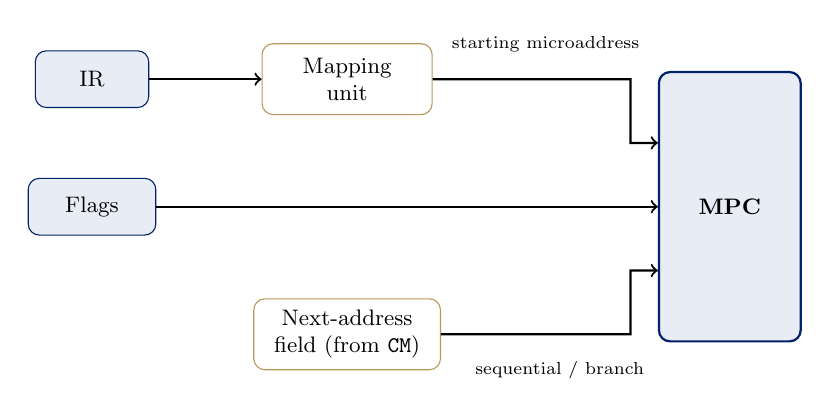
\begin{tikzpicture}[scale=0.90, transform shape,
        every node/.style={font=\small}]
      \node[draw=primary-blue, fill=light-bg, rounded corners,
            minimum width=1.6cm, minimum height=0.8cm, align=center]
            (IR) at (0,1.8) {IR};
      \node[draw=primary-gold, fill=white, rounded corners,
            minimum width=2.4cm, minimum height=1.0cm, align=center]
            (MAP) at (3.6,1.8) {Mapping\\unit};
      \draw[->, thick] (IR.east) -- (MAP.west);
      \node[font=\scriptsize] at (6.4,2.3) {starting microaddress};
      \node[draw=primary-blue, fill=light-bg, rounded corners,
            minimum width=1.8cm, minimum height=0.8cm, align=center]
            (FLAGS) at (0,0) {Flags};
      \node[draw=primary-gold, fill=white, rounded corners, text width=2.4cm,
            minimum height=1.0cm, align=center]
            (NEXT) at (3.6,-1.8) {Next-address field (from \texttt{CM})};
      \node[font=\scriptsize] at (6.6,-2.3) {sequential / branch};
      \node[draw=primary-blue, thick, fill=light-bg, rounded corners,
            minimum width=2.0cm, minimum height=3.8cm, align=center]
            (MPC) at (9.0,0) {\textbf{MPC}};
      \draw[->, thick] (MAP.east) -- (7.6,1.8) |- (MPC.west |- 0,0.9);
      \draw[->, thick] (FLAGS.east) -- (7.6,0) |- (MPC.west |- 0,0);
      \draw[->, thick] (NEXT.east) -- (7.6,-1.8) |- (MPC.west |- 0,-0.9);
    \end{tikzpicture}
  \end{center}
  Flags let a control word's next-address field \emph{branch} rather than
  simply advance --- how a conditional instruction (e.g.\ a compare-and-jump)
  selects between two successors \cite{Mano1993_computer_system_architecture}.
\end{frame}

\begin{frame}{Worked Trace Revisited: Where \texttt{MPC} Points}
  \footnotesize
  \begin{tabular}{@{}cccl@{}}
    \toprule
    \textbf{Step} & \textbf{MPC value} & \textbf{CM row read} & \textbf{RTL} \\
    \midrule
    Fetch & mapped $\to 0$ & row 0 & $Y \gets [R2]$ \\
    $+1$ & 1 & row 1 & $Z \gets [Y] + [R3]$ \\
    $+1$ & 2 & row 2 (\textsc{End}) & $R1 \gets [Z]$, then remap on next fetch \\
    \bottomrule
  \end{tabular}
  \vspace{0.3cm}
  \key{This is the piece that plays \texttt{SC}'s role}: mapping plus the
  next-address field is what turns ``read row 0, then 1, then 2'' from
  something we listed by hand into something the circuit does on its own.
\end{frame}

\begin{frame}{Socratic Check: What If Mapping Were Missing?}
  \begin{alertblock}{Question}
    Suppose the mapping unit were removed and \texttt{MPC} always reset to 0
    after \textsc{End}. What breaks?
  \end{alertblock}
  \begin{itemize}
    \item Every instruction would execute \texttt{CM} row 0's microprogram
      --- whichever instruction happens to occupy that address --- regardless
      of what is actually in \texttt{IR}.
    \item Exactly like Week 6's missing $SC_{\text{clear}}$, this is not
      optional bookkeeping: mapping is what lets a shared \texttt{CM} serve
      \emph{every} instruction instead of just one.
  \end{itemize}
\end{frame}

\transitionslide{But different instructions need different micro-operations at each step --- how wide is one control word?}

% =============================================================================
% ACT 3 --- HORIZONTAL VS. VERTICAL ENCODING
% =============================================================================
\section{Horizontal vs.\ Vertical Encoding}

\begin{frame}{The Missing Piece: How Wide Is a Control Word?}
  \begin{block}{Socratic question}
    Our worked microprogram used about eight distinct signals ($R2_{\text{out}}$,
    $R3_{\text{out}}$, $Y_{\text{in}}$, ALU$=$add, $Z_{\text{in}}$,
    $Z_{\text{out}}$, $R1_{\text{in}}$, \textsc{End}). A real ISA has dozens to
    hundreds. Does every control word need one bit \emph{per signal}, even
    though only a handful are ever active at once?
  \end{block}
  This is a genuine width-vs.-simplicity trade-off, and it has a name:
  \key{horizontal} vs.\ \key{vertical} microinstruction encoding.
\end{frame}

\begin{frame}{Definition: Horizontal Microinstruction}
  \begin{block}{Horizontal encoding}
    One bit per control signal. Bit $k$ of the control word \emph{is}
    $X_{\text{in}}$ (or $R2_{\text{out}}$, or \textsc{End}) directly ---
    reading the word out of \texttt{CM} \emph{is} asserting the signals, with
    no further logic in between.
  \end{block}
  \begin{itemize}
    \item \good{Pro}: no decode delay --- signals are valid the instant
      \texttt{CM} is read, same cycle.
    \item \bad{Con}: the word is as wide as the number of signals in the whole
      machine, and most bits are 0 in any given row.
  \end{itemize}
\end{frame}

\begin{frame}{Definition: Vertical Microinstruction}
  \begin{block}{Vertical encoding}
    Signals that are mutually exclusive (e.g.\ ``which register drives the
    bus this cycle'' has exactly one answer) are grouped into a small
    \emph{encoded field}. A \textbf{decoder} between \texttt{CM} and the
    datapath expands each field back into the actual one-hot signal.
  \end{block}
  \begin{itemize}
    \item \good{Pro}: far narrower control word --- $n$ mutually-exclusive
      signals need only $\lceil \log_2 n \rceil$ bits, not $n$.
    \item \bad{Con}: the decoder is on the critical path --- signals are valid
      one decode delay \emph{after} \texttt{CM} is read, not the same instant.
  \end{itemize}
\end{frame}

\begin{frame}{Side by Side: Encoding Our Worked Example}
  \begin{columns}[T]
    \begin{column}{0.48\textwidth}
      \centering \textbf{Horizontal} (row 1: $T_2$) \\[0.15cm]
      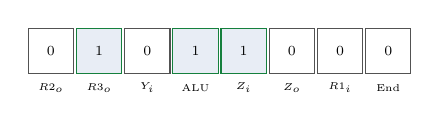
\begin{tikzpicture}[scale=0.72, transform shape,
          every node/.style={font=\scriptsize}]
        % Diagram: 8 individual 1-bit fields, one per signal, only the two
        % active this row shaded positive; rest shown as 0 in neutral outline.
        % Coordinates: (x, y) -- one row of unit-width boxes at y=0,
        %   x = 0..7 (0.8cm pitch), labels for the active bits above.
        \foreach \i/\lab/\val in {0/{$R2_{o}$}/0, 1/{$R3_{o}$}/1, 2/{$Y_{i}$}/0,
            3/{ALU}/1, 4/{$Z_{i}$}/1, 5/{$Z_{o}$}/0, 6/{$R1_{i}$}/0, 7/{End}/0} {
          \ifnum\val=1
            \node[draw=positive, fill=light-bg, minimum width=0.8cm,
                  minimum height=0.8cm] at (\i*0.85,0) {1};
          \else
            \node[draw=neutral, fill=white, minimum width=0.8cm,
                  minimum height=0.8cm] at (\i*0.85,0) {0};
          \fi
          \node[font=\tiny] at (\i*0.85,-0.65) {\lab};
        }
      \end{tikzpicture}
      \vspace{0.2cm}
      \muted{8 bits, one per signal --- read directly, no decoder.}
    \end{column}
    \begin{column}{0.48\textwidth}
      \centering \textbf{Vertical} (row 1: $T_2$) \\[0.15cm]
      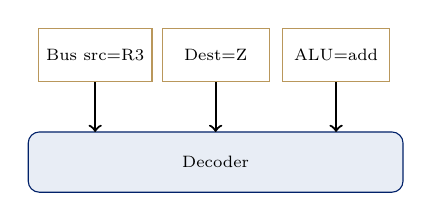
\begin{tikzpicture}[scale=0.85, transform shape,
          every node/.style={font=\scriptsize}]
        % Diagram: 3 encoded fields (bus source [2b], destination [2b],
        % ALU op [2b]) at y=0, then a decoder box below expanding them.
        % Coordinates: (x,y)
        \node[draw=primary-gold, fill=white, minimum width=1.6cm,
              minimum height=0.8cm] (F1) at (0,0) {Bus src$=$R3};
        \node[draw=primary-gold, fill=white, minimum width=1.6cm,
              minimum height=0.8cm] (F2) at (1.8,0) {Dest$=$Z};
        \node[draw=primary-gold, fill=white, minimum width=1.6cm,
              minimum height=0.8cm] (F3) at (3.6,0) {ALU$=$add};
        \node[draw=primary-blue, fill=light-bg, rounded corners,
              minimum width=5.6cm, minimum height=0.9cm, align=center]
              (DEC) at (1.8,-1.6) {Decoder};
        \draw[->, thick] (F1.south) -- (F1.south |- 0,-1.15);
        \draw[->, thick] (F2.south) -- (F2.south |- 0,-1.15);
        \draw[->, thick] (F3.south) -- (F3.south |- 0,-1.15);
      \end{tikzpicture}
      \vspace{0.2cm}
      \muted{3 fields ($\approx$6 bits) --- needs a decode step before signals
      are valid.}
    \end{column}
  \end{columns}
\end{frame}

\begin{frame}{Horizontal vs.\ Vertical: Trade-offs}
  \begin{block}{Width vs.\ speed}
    \begin{itemize}
      \item \good{Horizontal}: no decode delay, but \texttt{CM} width grows
        linearly with the number of signals in the machine --- at real-ISA
        scale, 100--400 bits per row is typical.
      \item \good{Vertical}: \texttt{CM} width shrinks to
        $\sim\!\log_2$(signals per group), summed across groups --- but every
        control word pays a decoder's worth of extra delay before the
        datapath sees valid signals.
      \item Our toy example (8 bits $\to$ $\approx$6 bits) barely shows the
        gain --- the saving compounds with instruction-set size, which is
        exactly where hardwired control's design cost was exploding.
    \end{itemize}
  \end{block}
\end{frame}

\transitionslide{Put the two new hardware pieces together --- what does the full control unit look like now?}

% =============================================================================
% ACT 4 --- TRADE-OFFS AND SYNTHESIS
% =============================================================================
\section{Trade-offs and Synthesis}

\begin{frame}{Full Microprogrammed Control Unit Block Diagram}
  \begin{center}
    % Diagram: capstone assembly -- IR feeds mapping unit (starting address);
    % Flags feed the branch decision; both converge into MPC; MPC feeds CM;
    % CM's control-word output splits into control signals (via an optional
    % decoder, folded into the "Control signals" box for vertical encoding)
    % and a next-address field that feeds back into MPC. Deliberately mirrors
    % Week 6's capstone layout (IR/Flags/Clock -> matrix -> outputs ->
    % feedback to SC) so the two designs read as structural twins.
    % Coordinates: (x, y)
    %   IR at (0, 2.2); Mapping unit at (3.2, 2.2)
    %   Flags at (0, 0.7); Clock at (0, -0.8) (feed MPC directly)
    %   MPC at (6.0, 0.7), tall enough to receive IR/Flags/Clock rows
    %   CM (large) at (9.6, 0.7)
    %   Control signals output at (13.4, 1.6); next-address feedback at
    %     (13.4, -0.2) looping back down to MPC
    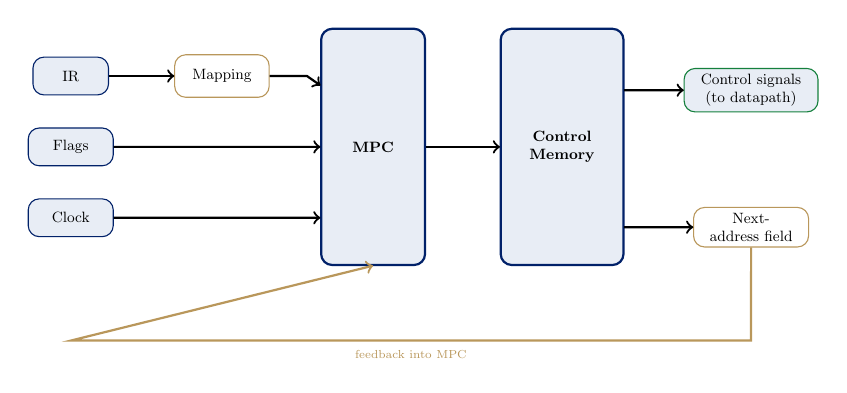
\begin{tikzpicture}[scale=0.60, transform shape,
        every node/.style={font=\small}]
      \node[draw=primary-blue, fill=light-bg, rounded corners,
            minimum width=1.6cm, minimum height=0.8cm, align=center]
            (IR) at (0,2.2) {IR};
      \node[draw=primary-gold, fill=white, rounded corners,
            minimum width=2.0cm, minimum height=0.9cm, align=center]
            (MAP) at (3.2,2.2) {Mapping};
      \draw[->, thick] (IR.east) -- (MAP.west);
      \node[draw=primary-blue, fill=light-bg, rounded corners,
            minimum width=1.8cm, minimum height=0.8cm, align=center]
            (FLAGS) at (0,0.7) {Flags};
      \node[draw=primary-blue, fill=light-bg, rounded corners,
            minimum width=1.8cm, minimum height=0.8cm, align=center]
            (CLK) at (0,-0.8) {Clock};
      \node[draw=primary-blue, thick, fill=light-bg, rounded corners,
            minimum width=2.2cm, minimum height=5.0cm, align=center]
            (MPC) at (6.4,0.7) {\textbf{MPC}};
      \draw[->, thick] (MAP.east) -- (5.0,2.2) -- (MPC.west |- 0,2.0);
      \draw[->, thick] (FLAGS.east) -- (5.0,0.7) -- (MPC.west |- 0,0.7);
      \draw[->, thick] (CLK.east) -- (5.0,-0.8) -- (MPC.west |- 0,-0.8);
      \node[draw=primary-blue, thick, fill=light-bg, rounded corners,
            minimum width=2.6cm, minimum height=5.0cm, align=center]
            (CM) at (10.4,0.7) {\textbf{Control}\\\textbf{Memory}};
      \draw[->, thick] (MPC.east) -- (CM.west);
      \node[draw=positive, fill=light-bg, rounded corners, text width=2.6cm,
            minimum height=0.8cm, align=center]
            (OUT1) at (14.4,1.9) {Control signals (to datapath)};
      \draw[->, thick] (CM.east |- 0,1.9) -- (OUT1.west);
      \node[draw=primary-gold, fill=white, rounded corners, text width=2.2cm,
            minimum height=0.8cm, align=center]
            (OUT2) at (14.4,-1.0) {Next-address field};
      \draw[->, thick] (CM.east |- 0,-1.0) -- (OUT2.west);
      \draw[->, thick, primary-gold] (OUT2.south) -- (14.4,-3.4) -- (0,-3.4) -- (0,-3.4) -- (MPC.south);
      \node[font=\scriptsize, primary-gold] at (7.2,-3.7) {feedback into MPC};
    \end{tikzpicture}
  \end{center}
  \cite{Mano1993_computer_system_architecture,Hamacher2002_computer_organization}
\end{frame}

\begin{frame}{Socratic Check: Adding a New Instruction}
  \begin{alertblock}{Question}
    Recall Week 6: adding \texttt{MUL} meant a new opcode-decoder line
    \emph{and} rewiring an AND gate into an existing OR gate on the chip.
    What does adding \texttt{MUL} cost here?
  \end{alertblock}
  \begin{itemize}
    \item Write \texttt{MUL}'s control words into \emph{unused} rows of
      \texttt{CM} --- no new gates.
    \item Extend the mapping unit with one more (opcode $\to$ starting
      microaddress) entry --- typically itself a small memory/table, not
      hand-derived logic.
    \item The chip's gates do not change at all; only the contents of a
      memory do.
  \end{itemize}
\end{frame}

\begin{frame}{Microprogrammed Control: Trade-offs}
  \begin{block}{Flexibility vs.\ speed}
    \begin{itemize}
      \item \good{Pro}: new or modified instructions are a memory rewrite,
        not a redesign --- even a bug fix in an already-fabricated CPU can
        ship as a microcode patch (real x86 chips do exactly this).
      \item \good{Pro}: the state table \emph{is} the design --- no
        hand-derived Boolean equations to re-verify.
      \item \bad{Con}: every control step costs a memory read (and a decode
        step, if vertical) --- strictly slower per cycle than hardwired's
        pure combinational logic.
      \item \bad{Con}: \texttt{CM} itself is extra hardware that hardwired
        control does not need at all.
    \end{itemize}
  \end{block}
\end{frame}

\begin{frame}{Hardwired vs.\ Microprogrammed: Head to Head}
  \footnotesize
  \begin{tabular}{@{}lll@{}}
    \toprule
    & \textbf{Hardwired (Week 6)} & \textbf{Microprogrammed (this week)} \\
    \midrule
    Speed per step & Fastest --- pure gates & Slower --- memory read (+ decode) \\
    Adding an instruction & New/re-wired gates & New \texttt{CM} rows \\
    Design method & Derive Boolean equations & Write down control words \\
    Typical fit & Small, fixed, speed-critical ISAs (RISC) & Large, evolving ISAs (classical CISC) \\
    \bottomrule
  \end{tabular}
  \vspace{0.3cm}
  \key{Same control problem, two implementations} --- the choice trades raw
  speed against design and maintenance cost, exactly the pattern Weeks 5--6
  already established for datapaths.
\end{frame}

\begin{frame}{The Three Threads Meet}
  \begin{block}{Every design choice moves cost somewhere else on the chip}
    \begin{itemize}
      \item \textbf{Bus organization (Week 5):} single-bus needs 3 control
        steps for our trace; three-bus needs 1 --- fewer steps, more wiring.
      \item \textbf{Control-unit style (Weeks 6--7):} hardwired is fastest per
        step but rigid; microprogrammed is slower per step but just a memory
        rewrite to change.
      \item \textbf{Encoding width (this week):} horizontal avoids decode
        delay but costs \texttt{CM} width; vertical shrinks \texttt{CM} but
        adds a decoder to the critical path.
    \end{itemize}
  \end{block}
  None of these is free --- every one trades cycle time, design effort, or
  raw hardware for one of the other two.
\end{frame}

\begin{frame}{Bridge to Week 8}
  \begin{exampleblock}{From controlling the chip to controlling the world}
    Weeks 6--7 answered ``how does the CPU decide what \emph{itself} does,
    every cycle?'' Week 8 asks the next question: how does the CPU decide
    what \emph{outside} devices --- keyboards, disks, printers --- do, and
    when?
  \end{exampleblock}
  \begin{itemize}
    \item I/O devices are far slower than the CPU --- naively waiting for one
      wastes thousands of cycles.
    \item Interrupts, polling, DMA, and I/O processors are four different
      answers to ``who watches the device, and what happens when it's ready?''
  \end{itemize}
\end{frame}

\begin{frame}{Summary}
  \begin{itemize}
    \item \key{Control word (microinstruction)} $=$ one stored row of control
      signals plus next-address information; a \key{microprogram} is the
      ordered sequence implementing one instruction.
    \item \key{Control memory (\texttt{CM})} $+$ \key{microprogram counter
      (\texttt{MPC})} replace the control matrix and \texttt{SC}: \texttt{MPC}
      addresses \texttt{CM}, whose output is the control word.
    \item \key{Address sequencing}: a \textbf{mapping} unit loads \texttt{MPC}
      with an instruction's starting microaddress; each control word's
      next-address field advances or branches \texttt{MPC} thereafter.
    \item \key{Horizontal} microinstructions (one bit per signal, no decode
      delay) vs.\ \key{vertical} (encoded fields, decoder required, narrower
      words) trade width against speed.
    \item \key{Hardwired vs.\ microprogrammed}: same control problem, opposite
      trade-offs --- speed and rigidity vs.\ a memory-read delay and
      easy modification.
  \end{itemize}
\end{frame}

\begin{frame}{References}
  \footnotesize
  \bibliographystyle{plain}
  \bibliography{../../Bibliography_base}
\end{frame}

\end{document}
